\documentclass[11pt]{article}
\usepackage[T1]{fontenc}
\usepackage{lmodern}
\usepackage[margin=1in]{geometry}
\usepackage{amsmath,amssymb,amsthm,mathtools,mathrsfs}
\usepackage{booktabs,longtable,array,enumitem,graphicx,xcolor,microtype,xurl}
\usepackage{fancyhdr}
\usepackage[colorlinks=true,linkcolor=blue!40!black,citecolor=blue!40!black,urlcolor=blue!50!black]{hyperref}
\usepackage{bookmark}
\definecolor{ink}{RGB}{25,45,65}
\definecolor{accent}{RGB}{20,91,120}
\newtheorem{theorem}{Theorem}[section]
\newtheorem{proposition}[theorem]{Proposition}
\newtheorem{lemma}[theorem]{Lemma}
\newtheorem{corollary}[theorem]{Corollary}
\theoremstyle{definition}
\newtheorem{definition}[theorem]{Definition}
\newtheorem{conjecture}[theorem]{Conjecture}
\theoremstyle{remark}
\newtheorem{remark}[theorem]{Remark}
\newtheorem{example}[theorem]{Example}
\DeclareMathOperator{\Li}{Li}
\DeclareMathOperator{\Repart}{Re}
\DeclareMathOperator{\Impart}{Im}
\DeclareMathOperator{\Res}{Res}
\newcommand{\ii}{\mathrm{i}}
\newcommand{\Q}{\mathbb Q}
\newcommand{\C}{\mathbb C}
\newcommand{\E}{\mathbb E}
\newcommand{\Z}{\mathbb Z}
\newcommand{\dd}{\,\mathrm d}
\newcommand{\eps}{\varepsilon}
\newcommand{\smallO}{\mathrm O}
\numberwithin{equation}{section}
\setcounter{tocdepth}{2}
\setlength{\headheight}{14pt}
\pagestyle{fancy}
\fancyhf{}
\fancyhead[L]{\small\textcolor{ink}{Polylogarithm arithmetic bridges}}
\fancyhead[R]{\small\textcolor{ink}{Sharp remainders and exact reductions}}
\fancyfoot[C]{\thepage}
\emergencystretch=3em
\hypersetup{pdftitle={Sharp Remainders and Exact Reductions in Polylogarithm Arithmetic Bridges},pdfauthor={Research continuation for the ProveIt Polylogarithms project with OpenAI assistance}}
\title{\textcolor{ink}{Sharp Remainders and Exact Reductions\\in Polylogarithm Arithmetic Bridges}\\[7pt]
\large Log-gamma moments, Herglotz derivatives, and a Gaussian relation obstruction}
\author{A research continuation for the ProveIt Polylogarithms project\\
\small with OpenAI assistance}
\date{10 October 2026}
\begin{document}
\maketitle
\begin{abstract}
We continue the Polylogarithms programme with two quantitative asymptotic
developments and exact algebraic support. For the classical factorial
expansion of log-gamma moments, we identify the coefficient-generating inverse,
prove its square-root singularity and complete late-coefficient expansion,
and derive an asymptotic error equal to half the first omitted term at the
least-term scale, including two correction terms. For normalized high
derivatives of the Herglotz function, an exact two-term expression has an
explicit remainder smaller than every power, with a stretched-exponential
bound and an explicit oscillatory leading term. A finite rational algorithm gives all derivatives at positive rational
arguments in Hurwitz-zeta, hence depth-one cyclotomic, coordinates. A sparse
linear witness and all-weight dimension theorems explain a limitation of
a specified depth-two relation presentation in the Gaussian \(S_4\) problem.
A new weight-seven harmonic-sum reduction is proposed with two independent
high-precision checks and an exact rational residual bound of \(10^{-260}\).
Finally, we correct the manuscript's description of
the cubic log-gamma moment: a Tornheim--Witten derivative evaluation is
classical, and we rederive it with convergence proofs and a reproducible
evaluator. Every new claim is distinguished from classical input, formal
algebra, numerical corroboration, and the conjectures left unresolved.
\end{abstract}
\tableofcontents
\newpage
\section{Scope, status, and principal results}
\label{sec:introduction}

The ProveIt Polylogarithms manuscript~\cite{ProveIt} organizes a large collection of
functional equations, special values, experimental reductions, and
arithmetic bridges. This continuation concentrates on a connected part
of that programme: logarithmic gamma moments, Herglotz derivatives, and
depth-two cyclotomic polylogarithms. The common methodological question is
how to turn a useful formal representation into a statement with
controlled errors or a precisely specified algebraic meaning.

The source baseline is commit
\begin{center}\small
\texttt{78f9e5df05eb0abb16c89fb00b9e89403598bd17}
\end{center}
of \nolinkurl{VladimirReshetnikov/ProveIt}. We concentrate on Chapters~4, 7, 9,
and~10 in \nolinkurl{Analysis/Polylogarithms/docs/manuscript}.
We also inspected the existing October continuations on alternating
harmonic sums, corpus corrections, rational-grid distribution ranks,
Stieltjes derivatives, and Herglotz obstructions. The accompanying source
manifest records the examined files. This article proposes additions and
corrections; it does not modify the upstream repository.

\subsection{What is proved here}

There are three principal developments.

First, the classical moment expansion
\[
 \frac1{n!}\int_0^1\log^n\Gamma(x)\dd x
 \sim\sum_{k\geq1}\frac{(-1)^{k-1}b_k}{k^n}
\]
has coefficients that grow exponentially. We identify their precise
growth and prove a sharp error law when the number of retained terms
grows linearly with \(n\). At the least-term scale the actual error is
asymptotic to \emph{one half of the first omitted term}; the article
computes two correction terms. This is stronger than a fixed-length
asymptotic expansion or a heuristic minimum-term estimate. The proof
requires a local analytic continuation of an inverse gamma branch and a
uniform estimate for a Taylor remainder across its circle of convergence.

Second, for
\[
 F(x)=\sum_{n\geq1}\frac{\psi(nx)-\log(nx)}n,\qquad
 D_r(x)=\frac{(-1)^{r+1}x^{r+1}}{r!}F^{(r)}(x),
\]
we show that
\[
 D_r(x)=\zeta(2)+\frac xr(\log x-H_{r-1})+E_r(x).
\]
The displayed elementary expression contains every algebraic order of
the large-\(r\) expansion. The remaining term admits a divisor-weighted
Tricomi-\(U\) representation, an effective gamma-factor bound, and an
explicit oscillatory asymptotic of size
\(r^{-3/4}e^{-2\sqrt{\pi r/x}}\). This yields the sharp exponential rate
and infinitely many positive and negative remainders. Here the derivative
order tends to infinity with \(x\) fixed; this is a different limit from
the familiar large-\(x\) Bernoulli expansion.

Third, we determine all-weight dimensions of a \emph{specified formal
presentation} of imaginary depth-two values at levels 3 and 4, after
quotienting by single products and the manuscript's \(g\)-family.
The Hilbert series are
\[
 \frac{t^5}{(1-t^2)(1-t^6)}
 \quad\hbox{and}\quad
 \frac{t^3}{(1-t^2)^2},
\]
respectively. A sparse functional separates the proposed Gaussian
\(S_4\) reduction from every row in that presentation. This identifies
what the chosen relation family cannot establish. It is not a proof of
linear independence of actual periods, and it is not a disproof of the
conjecture.

These results are supported by exact rational row calculations,
independent integral evaluations, precision increases, and explicit
analytic tail bounds. Their proofs do not depend on the numerical
checks.

\subsection{Classical input and attribution}

The moment expansion itself is due to Amdeberhan, Coffey, Espinosa,
Koutschan, Manna, and Moll~\cite{ACEMKM}. The square-root mechanism used
for its late coefficients is classical analytic combinatorics
\cite{FS}; its hypotheses and the constants are established here for
the inverse relevant to the moments. The growing-index remainder
analysis is the additional step.

Radchenko and Zagier~\cite{RZ} already state closure of all rational
Herglotz derivatives in depth-one cyclotomic polylogarithms. We supply
an explicit finite Bernoulli--Hurwitz coefficient formula and a
regularization calculation, not a new claim of closure. Their arithmetic
integral representations also underlie the divisor expansion used here.
Large-parameter asymptotics of Tricomi's function are classical
\cite{DLMF,Temme}; the effective sum over arithmetic sectors and its
high-derivative consequences are developed in this article.

The cubic log-gamma moment already has a Tornheim--Witten derivative
evaluation in Bailey--Borwein--Borwein~\cite{BBB}. We correct the
manuscript's open-problem wording and independently derive an equivalent
formula, including convergence details and an evaluator. A reduction to
a more restrictive prescribed basket of ordinary zeta derivatives
remains a different question.

The all-depth odd-harmonic-sum reflection and several low-weight
Gaussian reductions have already been proved in the repository's
continuations. We use them as established context. Likewise, a count of
survivors in a relation matrix is always tied to the exact relations
imposed. Zhao's broader work on cyclotomic relations~\cite{Zhao}
provides a useful warning against identifying a restricted row space
with the full algebra of periods.

\subsection{Conventions and verification levels}

Throughout, \(\log\) is the real logarithm on positive real arguments;
complex powers and the function \(U\) use principal branches unless
otherwise specified. We write \(H_n=\sum_{j=1}^n j^{-1}\), \(H_0=0\),
\(\psi=\Gamma'/\Gamma\), and
\[
 \Li_{a,b}(u,v)=\sum_{m>n\geq1}\frac{u^m v^n}{m^a n^b}.
\]
At convergent boundary points this is the ordinary value. When a
leading \(\Li_1(1)\) is required in a relation, the regularization is
specified explicitly. The Dirichlet beta and eta functions are
\[
 \beta(s)=\sum_{n\geq0}\frac{(-1)^n}{(2n+1)^s},\qquad
 \eta(s)=\sum_{n\geq1}\frac{(-1)^{n-1}}{n^s},
\]
with \(\eta(1)=\log2\) and \(G=\beta(2)\).

A theorem in this article has an analytic or exact algebraic proof.
A formal dimension is the dimension of the defined presentation.
An integer-relation candidate is a conjecture even when its residual
is extraordinarily small. Most numerical diagnostics use ordinary
high-precision arithmetic, so analytic truncation estimates are
distinguished from machine-certified rounding enclosures. The
\(S_6\) residual certificate instead uses exact rational arithmetic
with proved tails. No claim
of a formal proof-assistant verification is made.

The novelty assessment is relative to the pinned manuscript, the
inspected continuations, and the cited primary literature. The article
does not claim an exhaustive priority search. All statements presented
as theorems stand on their supplied proofs, independently of that
bibliographic qualification.


\section{Log-gamma moments: from a classical expansion to a sharp error law}
\label{sec:moments}

For \(n\geq 0\), write
\[
 M_n=\int_0^1\log^n\Gamma(x)\dd x,\qquad m_n=\frac{M_n}{n!}.
\]
The convention \(M_0=1\) is understood. The classical expansion of
Amdeberhan et al.~\cite{ACEMKM} is
\begin{equation}\label{eq:classical-moment}
 m_n\sim\sum_{k\geq1}\frac{(-1)^{k-1}b_k}{k^n},\qquad
 b_k=\frac1k[z^{k-1}]\Gamma(1-z)^k>0.
\end{equation}
Here and below an infinite asymptotic expansion means that its truncation
index is fixed before \(n\to\infty\). It does not assert convergence of the
infinite sum for any fixed \(n\). Our aim is to determine the growth of
\(b_k\), locate the least term, and prove the error when the truncation
index grows with \(n\).

\subsection{Inverse coordinates and residues}

Let \(g\) denote the inverse germ at zero of the entire reciprocal gamma
function:
\[
 \frac1{\Gamma(g(t))}=t,\qquad g(0)=0,\qquad g'(0)=1.
\]
For \(0\leq t\leq1\), use the real continuation with \(0\leq g(t)\leq1\).
It exists uniquely: \(\psi(x)<0\) for \(0<x\leq1\), because
\(\psi\) is increasing and \(\psi(1)=-\gamma<0\).
Thus \(1/\Gamma(x)\) is strictly increasing from 0 to 1 on this interval.
The inverse under discussion is not the increasing large-argument inverse
of \(\Gamma\).

\begin{proposition}[Inverse and Mellin descriptions]\label{prop:inverse}
With \(c_k=(-1)^{k-1}b_k\), the inverse germ satisfies
\begin{equation}\label{eq:g-series}
 g(t)=\sum_{k\geq1}c_kt^k,\qquad
 B(t):=-g(-t)=\sum_{k\geq1}b_kt^k=t\Gamma(1-B(t)).
\end{equation}
For \(n\geq1\),
\begin{equation}\label{eq:layercake}
 m_n=\frac1{(n-1)!}\int_0^\infty y^{n-1}g(e^{-y})\dd y.
\end{equation}
The function
\[
 \mathcal M(s)=\int_0^1\Gamma(x)^s\dd x,\qquad \Re s<1,
\]
continues meromorphically to \(\C\), has only simple poles at the
positive integers, and
\begin{equation}\label{eq:mgf-res}
 \Res_{s=k}\mathcal M(s)=-k c_k,\qquad
 [s^n]\mathcal M(s)=m_n.
\end{equation}
Every positive integer is an actual pole.
\end{proposition}

\begin{proof}
The inverse equation is \(g=t\Gamma(1+g)\). Lagrange inversion gives
\([t^k]g=k^{-1}[z^{k-1}]\Gamma(1+z)^k=c_k\).
The expansion
\begin{equation}\label{eq:phi}
 \Phi(z):=\Gamma(1-z)
 =\exp\left(\gamma z+\sum_{j\geq2}\frac{\zeta(j)}jz^j\right)
\end{equation}
has strictly positive coefficients. This proves the positivity in
\eqref{eq:classical-moment} and the equation for \(B\).
The function \(x\mapsto\log\Gamma(x)\) decreases from infinity to zero;
the measure of the set where it exceeds \(y\) is \(g(e^{-y})\).
The layer-cake formula for a nonnegative function gives
\eqref{eq:layercake}.

For the last assertion, set \(H(x,s)=\Gamma(1+x)^s\), using its analytic
logarithm for \(|x|<1\). Write
\(H(x,s)=\sum_{j\geq0}a_j(s)x^j\), with each \(a_j\) entire in \(s\).
Choose \(0<d<1\), split the integral at \(d\), and subtract a finite
Taylor polynomial on \([0,d]\). For every integer \(J\geq0\),
\begin{align}
 \mathcal M(s)
 &=\sum_{j=0}^J\frac{a_j(s)d^{j+1-s}}{j+1-s}
   +\int_0^d x^{-s}\left(H(x,s)-\sum_{j=0}^Ja_j(s)x^j\right)\dd x
   +\int_d^1\Gamma(x)^s\dd x. \label{eq:meromorphic}
\end{align}
The remainder integral is holomorphic in \(\Re s<J+2\), locally
uniformly there. Taking \(J\) arbitrarily large proves continuation.
At \(s=k\), the residue is \(-a_{k-1}(k)=-k c_k\), which is nonzero.
Differentiation under the original integral near \(s=0\) proves the
coefficient identity.
\end{proof}

Subtracting the first \(K\) polar parts \(k c_k/(k-s)\) from
\(\mathcal M\) leaves a function holomorphic in \(|s|<K+1\).
Cauchy's estimate, after subtracting one extra pole, consequently gives
the rigorous fixed-length version
\begin{equation}\label{eq:fixed-remainder}
 m_n=\sum_{k=1}^K\frac{c_k}{k^n}
       +\frac{c_{K+1}}{(K+1)^n}
       +O_{K,R}(R^{-n}),\qquad K+1<R<K+2.
\end{equation}
This recovers the classical expansion by a meromorphic argument; it is
not presented as a new asymptotic scale.

For exact coefficient generation, define \(a_0(s)=1\) and
\[
 a_j(s)=\frac{s}{j}\sum_{\ell=1}^j q_\ell a_{j-\ell}(s),\qquad
 q_1=\gamma,\quad q_\ell=\zeta(\ell)\quad(\ell\geq2).
\]
Then \(b_k=a_{k-1}(k)/k\). This recurrence involves only rational
arithmetic in the formal symbols \(\gamma,\zeta(2),\ldots\).
For example,
\begin{align*}
 b_1&=1,& b_2&=\gamma,&
 b_3&=\frac{3\gamma^2+\zeta(2)}2,\\
 b_4&=\frac{8\gamma^3+6\gamma\zeta(2)+\zeta(3)}3,\\
 b_5&=\frac{125\gamma^4}{24}
      +\frac{25\gamma^2\zeta(2)}4+\frac{5\gamma\zeta(3)}3
      +\frac{5\zeta(2)^2}{8}+\frac{\zeta(4)}4.
\end{align*}
These homogeneous polynomials have weight \(k-1\) under the formal
assignments \(\mathrm{wt}(\gamma)=1\) and
\(\mathrm{wt}(\zeta(j))=j\). No independence assumption is needed to
generate or verify them.

\subsection{The singularity that controls late coefficients}

\begin{theorem}[Late coefficients]\label{thm:late}
There is a unique \(\tau\in(0,1)\) satisfying \(\psi(-\tau)=0\).
Define
\begin{equation}\label{eq:constants}
 \rho=\frac{\tau}{\Gamma(1-\tau)},\qquad
 \Lambda=-\log\rho,\qquad
 C=\frac1{\sqrt{2\pi\psi'(-\tau)}}.
\end{equation}
Then \(B\) has radius of convergence \(\rho\), its only singularity on
that circle is \(\rho\), and it has a square-root expansion there.
In particular,
\begin{equation}\label{eq:late}
 b_k=C\rho^{-k}k^{-3/2}
       \left(1+\frac{d_1}{k}+O(k^{-2})\right).
\end{equation}
A complete expansion in powers of \(1/k\) exists. If
\(\kappa_j=((z\,\partial_z)^j\log\Phi(z))|_{z=\tau}\), so that
\(\kappa_1=1\), then
\begin{equation}\label{eq:d1}
 d_1=-\frac1{2\kappa_2}
      +\frac{\kappa_3}{2\kappa_2^2}
      +\frac{\kappa_4}{8\kappa_2^2}
      -\frac{5\kappa_3^2}{24\kappa_2^3}.
\end{equation}
Equivalently, with \(P=\psi'(-\tau)\), \(Q=\psi''(-\tau)\),
and \(R=\psi'''(-\tau)\),
\begin{equation}\label{eq:d1-polygamma}
 d_1=\frac{R}{8P^2}-\frac{5Q^2}{24P^3}.
\end{equation}
\end{theorem}

\begin{proof}
The characteristic equation for \(B=t\Phi(B)\) is
\(\tau\Phi'(\tau)=\Phi(\tau)\).
Since \(\Phi'/\Phi=-\psi(1-z)\), recurrence of the digamma function
turns this into \(\psi(-\tau)=0\).
Alternatively \(z\Phi'(z)/\Phi(z)=\gamma z+\sum_{j\geq2}\zeta(j)z^j\)
is strictly increasing from 0 to infinity on \((0,1)\), proving
existence and uniqueness. The function \(z/\Phi(z)\) increases up to
\(\tau\) and then decreases.

The power series solution has nonnegative coefficients and reaches
\(B(\rho)=\tau\). One elementary justification is to iterate
\(B_{j+1}=t\Phi(B_j)\), starting with \(B_0=0\), for \(0\leq t<\rho\);
monotonicity and the smaller real solution bound the iterates.
Monotone convergence and inversion give the limit at \(\rho\).
At the characteristic point,
\[
 \Phi''(\tau)/\Phi(\tau)
 =\psi'(1-\tau)+\psi(1-\tau)^2
 =\psi'(1-\tau)+\tau^{-2}=\psi'(-\tau)>0.
\]
Local inversion therefore gives
\begin{equation}\label{eq:puiseux}
 B(t)=\tau-\alpha\sqrt{1-t/\rho}+O(1-t/\rho),
 \qquad \alpha=\sqrt{\frac2{\psi'(-\tau)}}.
\end{equation}
There is a convergent Puiseux expansion, with integral and half-integral
powers.

For completeness, there are no other dominant singularities.
Absolute convergence at \(|t|=\rho\) follows from \(B(\rho)=\tau\).
If \(t\neq\rho\) lies on that circle, the positive coefficients of
\(t\) and \(t^2\) give \(|B(t)|<\tau\). Hence
\[
 |t\Phi'(B(t))|\leq\rho\Phi'(|B(t)|)<\rho\Phi'(\tau)=1.
\]
The analytic implicit-function theorem continues \(B\) across every such
point. Compactness, together with local square-root inversion at \(\rho\),
supplies a slit disk \(|t|<\rho+\epsilon\) with the sole cut issuing from
\(\rho\). This is the smooth implicit-function mechanism of
analytic combinatorics~\cite{FS}, with its hypotheses verified here.
Transfer of \((1-t/\rho)^{1/2}\) gives
\(C=\alpha/(2\sqrt\pi)\) and the full expansion.

We also give a direct computation of the first correction.
Lagrange's coefficient integral on \(|z|=\tau\) is
\[
 b_k=\frac{\tau\rho^{-k}}{2\pi k}
 \int_{-\pi}^{\pi}
 \exp\!\left(k\{\log\Phi(\tau e^{i\theta})-\log\Phi(\tau)-i\theta\}\right)
 e^{i\theta}\dd\theta.
\]
Positivity and aperiodicity make the modulus strictly smaller away from
\(\theta=0\). At zero the exponent is
\(-\kappa_2\theta^2/2-i\kappa_3\theta^3/6
 +\kappa_4\theta^4/24+\cdots\).
After \(\theta=u/\sqrt{k}\), Gaussian integration gives respectively
\(-1/(2\kappa_2)\), \(\kappa_3/(2\kappa_2^2)\),
\(\kappa_4/(8\kappa_2^2)\), and
\(-5\kappa_3^2/(24\kappa_2^3)\).
Also \(\kappa_2=\tau^2\psi'(-\tau)\), so the leading constant agrees
with \eqref{eq:constants}. Taylor expansion to any fixed order, with an
exponentially small outer arc, proves the complete saddle expansion.
\end{proof}

Numerical values, used only as orientation, are
\begin{align*}
 \tau&=0.5040830082644554092582693045333024989\ldots,\\
 \rho&=0.2821158090062980421537966006204637282\ldots,\\
 \Lambda&=1.2654376221108656133820359111654739922\ldots,\\
 C&=0.1334277613094452848960205705394178243\ldots,\\
 d_1&=0.3019628287812052411245866827164781138\ldots.
\end{align*}

\begin{corollary}[Divergence and least terms]\label{cor:least}
For every fixed \(n\), the terms of the infinite series in
\eqref{eq:classical-moment} eventually grow in magnitude and do not tend
to zero. Its smallest terms occur at
\[
 k=\frac{n+3/2}{\Lambda}+O(1).
\]
For any integer \(N\) with \(N\Lambda-n\) bounded,
\begin{equation}\label{eq:least-size}
 \frac{b_N}{N^n}
 =C\left(\frac{e\Lambda}{n+3/2}\right)^{n+3/2}
       (1+O(n^{-1})).
\end{equation}
\end{corollary}

\begin{proof}
Equation \eqref{eq:late} gives exponential growth \(\rho^{-k}\);
\(\rho<1\), for example because \(\Phi(\tau)>1\) and \(\tau<1\).
The full coefficient expansion gives
\[
 \log\frac{b_{k+1}/(k+1)^n}{b_k/k^n}
 =\Lambda-(n+3/2)\log(1+1/k)+O(k^{-2}).
\]
This changes sign in a bounded interval around the displayed value.
No fixed initial index can be a global minimum for large \(n\),
and the same ratio excludes the other ranges.
Finally, the function \(k\Lambda-(n+3/2)\log k\) has a stationary
point at \((n+3/2)/\Lambda\); a bounded shift changes it by \(O(n^{-1})\).
\end{proof}

\subsection{A uniform Taylor-remainder lemma}

The next statement is the key passage from fixed-order asymptotics to
optimal truncation. It explicitly crosses the radius of convergence on
the positive real axis; merely summing an infinite Taylor tail there
would be invalid.

\begin{lemma}[Uniform inverse remainder]\label{lem:inverse-remainder}
For some \(\delta>0\), uniformly for
\(t\in[\rho e^{-\delta},\rho e^\delta]\), put \(r=t/\rho\). Then
\begin{equation}\label{eq:inverse-remainder}
 \frac{g(t)-\sum_{k=1}^{N-1}c_kt^k}{c_Nt^N}
 =\frac1{1+r}+\frac{3r}{2N(1+r)^2}+O(N^{-2}).
\end{equation}
On each of the remaining real intervals
\(0<t\leq\rho e^{-\delta}\) and
\(\rho e^\delta\leq t\leq1\), the same normalized remainder is
bounded uniformly in \(N\) sufficiently large.
\end{lemma}

\begin{proof}
The preceding theorem gives a slit disk of continuation for \(g\),
with its only singularity at \(-\rho\).
Choose its outer radius \(R>\rho\), and then \(\delta>0\) so small that
\(\rho e^\delta<R\) and \(\rho e^\delta<1\).
Cauchy's integral formula for \(g(t)\), less its first \(N-1\)
Taylor terms, has kernel \(t^N/(z^N(z-t))\). Deform its contour to the
two banks of the negative cut and an outer contour.
The coefficient \(c_N\) uses kernel \(z^{-N-1}\).
On the cut \(z=-s\), the ratio of these kernels, after removing
\(t^N\), is
\[
 \frac{z}{z-t}=\frac{s}{s+t}.
\]
The jump of \(g\) at \(s=\rho\) is a nonzero constant times
\((s-\rho)^{1/2}(1+O(s-\rho))\), with a complete expansion.
The coefficient integral is thus a Watson-type endpoint integral
whose normalized variable \(u=(s-\rho)/\rho\) has
\[
 \langle u\rangle=\frac{3}{2N}+O(N^{-2}),
 \qquad \langle u^2\rangle=O(N^{-2}).
\]
These formulas follow directly by comparing
\(\int_0^\epsilon u^{j+1/2}(1+u)^{-N-1}\dd u\)
with its beta integral extended to infinity. Terms outside a fixed
small neighborhood of zero are exponentially smaller.
Expanding
\[
 \frac{s}{s+t}
 =\frac1{1+r}+\frac{r}{(1+r)^2}u+O(u^2)
\]
proves \eqref{eq:inverse-remainder}.
The outer contour contributes \(O(R^{-N})\) to the coefficient and
\(O((t/R)^N)\) to the remainder; after normalization these errors are
exponentially small uniformly on the stated compact \(t\)-interval.
This contour argument defines and estimates the actual analytic
remainder on both sides of \(t=\rho\).

It remains to bound the two outer real intervals.
The estimate \(b_k\asymp\rho^{-k}k^{-3/2}\) implies that, below
\(\rho e^{-\delta}\), the absolutely convergent tail is bounded by
a constant times \(b_Nt^N\). Above \(\rho e^\delta\), use
\[
 \sum_{k<N}\frac{b_kt^k}{b_Nt^N}
 \ll\sum_{k<N}(N/k)^{3/2}(\rho/t)^{N-k}.
\]
Splitting at \(k=N/2\) bounds this uniformly by a geometric series
plus an exponentially small term times a polynomial in \(N\).
Furthermore \(0\leq g(t)\leq1\), whereas \(b_Nt^N\) grows
exponentially uniformly on this interval. This proves the last claim.
\end{proof}

\subsection{Sharp optimal truncation}

\begin{theorem}[Half the first omitted term]\label{thm:optimal-moment}
Let \(n,N\) tend to infinity through positive integers with
\(\eta=N\Lambda-n\) in a fixed bounded interval. Then
\begin{equation}\label{eq:optimal-moment}
 \boxed{\displaystyle
 m_n-\sum_{k=1}^{N-1}\frac{(-1)^{k-1}b_k}{k^n}
 =\frac{(-1)^{N-1}b_N}{N^n}
 \left(\frac12+\frac{3-2\eta}{8N}+O(N^{-2})\right).}
\end{equation}
The \(O\)-constant is uniform for bounded \(\eta\).
The ratio in parentheses has a complete asymptotic expansion in
\(1/N\), with coefficients computable from the local inverse expansion
and gamma moments.
In particular, taking the nearest integer to \((n+3/2)/\Lambda\)
gives a rigorously justified least-term approximation. The error
eventually has the sign of the first omitted term and is asymptotic
to one half of that term.
\end{theorem}

\begin{proof}
Subtract the finite sum under \eqref{eq:layercake}, using
\[
 \frac1{(n-1)!}\int_0^\infty y^{n-1}e^{-ky}\dd y=k^{-n}.
\]
With \(Y\) having the gamma density
\(N^ny^{n-1}e^{-Ny}/(n-1)!\), the error divided by \(c_N/N^n\) is
the expectation of the normalized inverse remainder at \(t=e^{-Y}\).

The gamma distribution concentrates at \(\Lambda\):
\[
 \E Y=\frac nN=\Lambda-\frac\eta N,\qquad
 \operatorname{Var}Y=\frac n{N^2}.
\]
For every fixed small \(\delta>0\), its probability outside
\([\Lambda-\delta,\Lambda+\delta]\) is \(O(e^{-a_\delta N})\).
This follows from its moment-generating function
\((1-u/N)^{-n}\) and Chernoff's inequality.
The uniform outer bounds in Lemma~\ref{lem:inverse-remainder}
therefore make the outer contribution exponentially small.

On the middle interval, the leading kernel is
\[
 L(Y-\Lambda)=\frac1{1+e^{\Lambda-Y}},\qquad
 L(v)=\frac12+\frac v4-\frac{v^3}{48}+O(v^4).
\]
Writing \(V=Y-\Lambda\), its centered gamma moments give
\[
 \E V=-\frac\eta N,\qquad
 \E V^3=O(N^{-2}),\qquad \E V^4=O(N^{-2}),
\]
uniformly for bounded \(\eta\). Thus
\(\E L(V)=1/2-\eta/(4N)+O(N^{-2})\).
It is essential here to use the signed third moment; an absolute
cubic bound alone would lose half a power.
The correction kernel in \eqref{eq:inverse-remainder} is
\[
 \frac{3e^{-V}}{2N(1+e^{-V})^2}.
\]
Its value at zero is \(3/(8N)\), and its first derivative vanishes
there, so its expectation is \(3/(8N)+O(N^{-2})\).
Adding these terms proves \eqref{eq:optimal-moment}.
The contour calculation and the Taylor/gamma-moment calculation can
both be continued to arbitrary fixed order. Gamma central moments
are polynomials in \(n\) and \(N^{-1}\); their parity and degree give
integer powers of \(N^{-1}\).
\end{proof}

The theorem strengthens the classical expansion in two ways.
It allows \(N\) to grow linearly with \(n\), and it estimates the
actual error after truncation. The least-term estimate alone would
not justify either conclusion. No global sign assertion for every
\(n,N\) is needed.

\begin{corollary}[Second correction]\label{cor:moment-second}
Under the hypotheses of Theorem~\ref{thm:optimal-moment}, the normalized
error has the more precise expansion
\begin{align}
 \frac{m_n-\sum_{k<N}c_k/k^n}{c_N/N^n}
 &=\frac12+\frac{3-2\eta}{8N}\notag\\
 &\quad+\frac1{N^2}
 \left(\frac{d_1}{4}+\frac{\Lambda(6\eta-13)}{96}\right)
 +O(N^{-3}).\label{eq:moment-second}
\end{align}
\end{corollary}

\begin{proof}
Here are the additional local coefficients, so that the assertion is
independently reproducible. Let \(v=B-\tau\), and use \(P,Q,R\)
from \eqref{eq:d1-polygamma}. The characteristic inverse satisfies
\[
 \log\frac{B/\Gamma(1-B)}{\rho}
 =-\frac{P}{2}v^2+\frac{Q}{6}v^3-\frac{R}{24}v^4+O(v^5).
\]
Putting \(w=\sqrt{1-t/\rho}\) and
\(\alpha=\sqrt{2/P}\), inversion gives
\[
 B(t)=\tau-\alpha w+\frac{Q}{3P^2}w^2+\mu w^3+O(w^4),
 \qquad
 D:=\frac{\mu}{\alpha}
 =-\frac14+\frac{R}{12P^2}-\frac{5Q^2}{36P^3}.
\]
Thus the positive cut density for \(B\) is
\((\alpha/\pi)u^{1/2}(1+Du+O(u^2))\), where \(u=t/\rho-1\).
Transfer gives \(d_1=3/8+3D/2\), proving
\eqref{eq:d1-polygamma} as well. The normalized endpoint moments are
\[
 \langle u\rangle=\frac{3}{2N}
       +\frac{9/4+3D/2}{N^2}+O(N^{-3}),\qquad
 \langle u^2\rangle=\frac{15}{4N^2}+O(N^{-3}),\qquad
 \langle u^3\rangle=O(N^{-3}).
\]
They follow from beta integrals and the displayed cut density.
The coefficient of \(N^{-2}\) in the inverse remainder at \(r=t/\rho\)
is therefore
\[
 K_2(r)=\frac{r}{(1+r)^2}\left(\frac94+\frac{3D}{2}\right)
                    -\frac{15r}{4(1+r)^3},\qquad K_2(1)=d_1/4.
\]
For the gamma average, put
\(K_1(v)=3e^{-v}/[2(1+e^{-v})^2]\) and \(V=Y-\Lambda\).
Taylor expansion through degree five, using
\(\E|V|^6=O(N^{-3})\), gives
\[
 \E L(V)=\frac12-\frac{\eta}{4N}
       +\frac{\Lambda(3\eta-2)}{48N^2}+O(N^{-3}),\qquad
 \E K_1(V)=\frac38-\frac{3\Lambda}{32N}+O(N^{-2}).
\]
For example \(\E V^3=\Lambda(2-3\eta)N^{-2}+O(N^{-3})\);
the signed fifth moment is \(O(N^{-3})\).
Also \(\E K_2(e^{-V})=K_2(1)+O(N^{-1})\).
The uniform outer bound again makes all outer contributions
exponentially small. Combining the three terms proves
\eqref{eq:moment-second}.
\end{proof}

\begin{figure}[t]
 \centering
 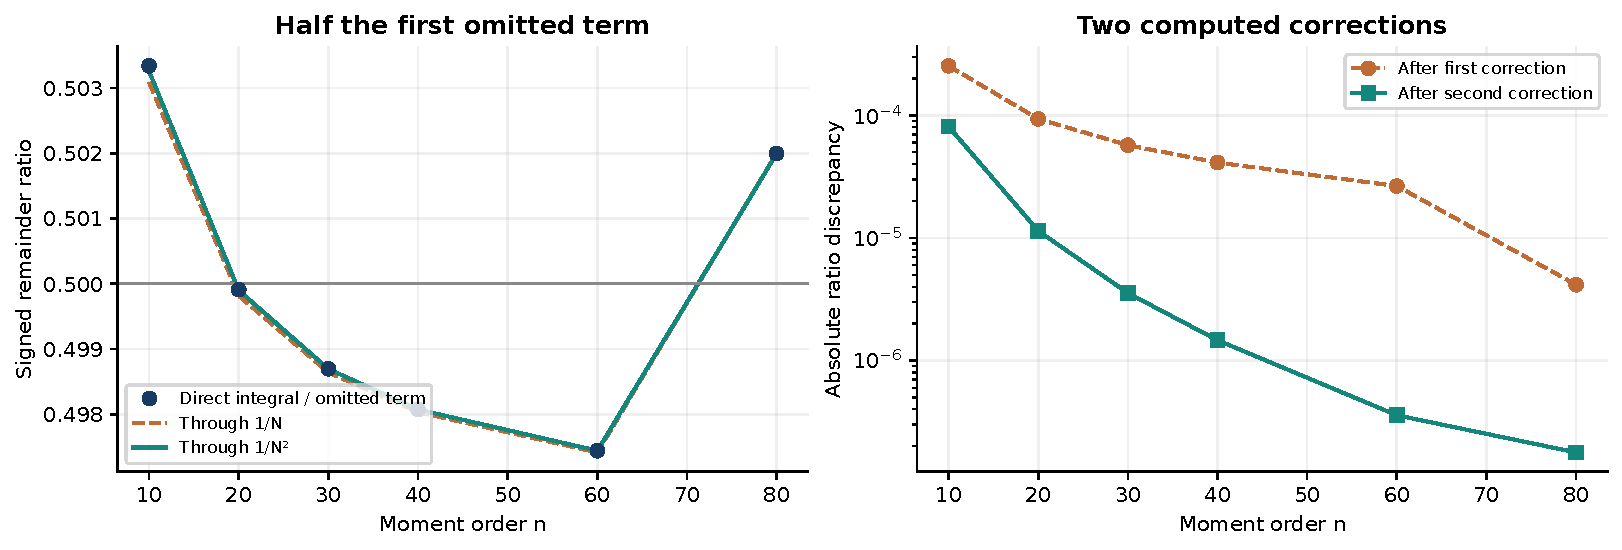
\includegraphics[width=\textwidth]{figures/moment_remainders.pdf}
 \caption{The signed error divided by the first omitted term, at a
 truncation near \((n+3/2)/\Lambda\). The first-correction formula tracks
 the small changes caused by rounding the truncation index. The plot is
 numerical corroboration; Theorem~\ref{thm:optimal-moment} supplies the proof.}
 \label{fig:moments}
\end{figure}

\subsection{A convergent identity with an explicit tail bound}

An asymptotic series should not be used as an infinite exact sum.
The same inverse coordinate gives an exact convergent alternative.

\begin{proposition}[Cutoff identity]\label{prop:cutoff}
For \(n\geq1\) and \(Y>\Lambda\),
\begin{equation}\label{eq:cutoff}
 m_n=\frac1{(n-1)!}\int_0^Y y^{n-1}g(e^{-y})\dd y
      +\sum_{k\geq1}\frac{c_k}{k^n}Q(n,kY),
 \qquad
 Q(n,z)=e^{-z}\sum_{j=0}^{n-1}\frac{z^j}{j!}.
\end{equation}
The sum is absolutely convergent. If \(Y>\log4\), the absolute tail
after \(k=K\) is at most
\begin{equation}\label{eq:cutoff-bound}
 \frac{(4e^{-Y})^{K+1}}{2(1-4e^{-Y})}
 \sum_{j=0}^{n-1}\frac{Y^j}{j!(K+1)^{n-j}}.
\end{equation}
\end{proposition}

\begin{proof}
Split \eqref{eq:layercake} at \(Y\), substitute the convergent inverse
series on the tail, and integrate term by term.
The coefficient growth theorem proves absolute convergence.
For the elementary explicit bound, note that
\[
 \frac{1/2}{\Phi(1/2)}=\frac1{2\sqrt\pi}>\frac14.
\]
The smaller solution to \(B=t\Phi(B)\) at \(t=1/4\) is therefore
less than \(1/2\); equivalently \(B(1/4)<1/2\).
Positivity gives \(b_k\leq4^k/2\).
For \(k>K\) and \(j\leq n-1\), \(k^{j-n}\leq(K+1)^{j-n}\).
The geometric tail now gives \eqref{eq:cutoff-bound}.
\end{proof}

The numerical implementation uses ordinary high-precision arithmetic
and explicitly distinguishes analytic truncation bounds from interval
rounding bounds. Formula \eqref{eq:cutoff} is also suitable for a future
ball-arithmetic evaluator: the finite inverse integral and all constant
evaluations can be enclosed separately.


\section[Rational Herglotz derivatives and an exponentially small oscillation]{Rational Herglotz derivatives\\and an exponentially small oscillation}
\label{sec:herglotz}

Let
\[
 F(x)=\sum_{n\ge1}\frac{\psi(nx)-\log(nx)}n,\qquad
 D_r(x)=\frac{(-1)^{r+1}x^{r+1}}{r!}F^{(r)}(x)
 \quad(r\ge1, x>0).
\]
The all-orders assertion that rational jets reduce to depth-one cyclotomic
polylogarithms is already stated by Radchenko--Zagier~\cite{RZ}, immediately after
Proposition~4 of their preprint, p.~9. It must not be presented as a new
closure theorem. The explicit Bernoulli coefficient formula below gives a
constructive version; the large-order estimate and its effective remainder
bound are derived independently here. The limit considered below is derivative order tending to infinity at a fixed positive argument.

\subsection{An explicit finite rational-jet formula}

Write $B_j(X)$ for the Bernoulli polynomials with $B_1(X)=X-1/2$.
For positive integers $p,q$ (coprimality is unnecessary for this formula), put
\[
 c_{a,b}=\frac aq+\frac bp,\qquad
 d_{r,j}(a,b)=\binom rj B_{r-j}(1-b/p)
              -\mathbf1_{j=0}B_r(a/q),
\]
where $1\le a\le q$, $0\le b<p$, and $0\le j<r$.

\begin{theorem}[Finite Bernoulli--Hurwitz evaluator]\label{thm:rational-jets}
For $r\ge1$,
\begin{align*}
F^{(r)}(p/q)
={}&\frac{(-1)^{r+1}(r-1)!q^{r-1}}{p^{r+1}}
\left\{
\sum_{a=1}^{q}\sum_{b=0}^{p-1}
\left[-\psi(c_{a,b})+
 \sum_{j=0}^{r-1}d_{r,j}(a,b)\zeta(r+1-j,c_{a,b})\right]
\right.\\[-2pt]
&\hspace{50mm}\left.{}+pq\left(\frac1r-\gamma-\log q\right)
\right\}.
\end{align*}
In particular every Hurwitz zeta value in the formula has integer order
between $2$ and $r+1$; no spectral derivatives occur.
\end{theorem}

\begin{proof}
Use the classical integral representation (Radchenko--Zagier, eq.~(6))
\[
 F^{(r)}(x)=(-1)^{r+1}
 \int_0^\infty t^r\operatorname{Li}_{1-r}(e^{-xt})
 \left(\frac1{1-e^{-t}}-\frac1t\right)dt.
\]
After $t=qu$ introduce, initially for $\Re s>0$,
\[
 I(s)=\int_0^\infty u^{r+s}\operatorname{Li}_{1-r}(e^{-pu})
 \left(\frac1{1-e^{-qu}}-\frac1{qu}\right)du.
\]
The combined integral is holomorphic on $\Re s>-1$ since its integrand is
$O(u^{\Re s})$ at zero. In $\Re s>0$ the two terms can be integrated
separately, giving
\[
 I(s)=\Gamma(r+1+s)
 \sum_{n\ge1,m\ge0}\frac{n^{r-1}}{(pn+qm)^{r+1+s}}
 -\frac{\Gamma(r+s)}{qp^{r+s}}\zeta(1+s).
\]
Set $n=qk+a$, $m=p\ell+b$, and $h=k+\ell$. Faulhaber's identity gives
\[
 \sum_{k=0}^h(qk+a)^{r-1}
 =\frac{q^{r-1}}r
 \left[B_r(h+1+a/q)-B_r(a/q)\right].
\]
Writing $v=h+c_{a,b}$ expands the bracket as
$\sum_{j=0}^r d_{r,j}(a,b)v^j$, with $d_{r,r}=1$.
Consequently
\[
 \sum_{n\ge1,m\ge0}\frac{n^{r-1}}{(pn+qm)^{r+1+s}}
 =\frac{q^{r-1}}{r(pq)^{r+1+s}}
 \sum_{a,b}\sum_{j=0}^r d_{r,j}(a,b)
 \zeta(r+1+s-j,c_{a,b}).
\]
The $j=r$ terms have Laurent expansion
$\zeta(1+s,c)=s^{-1}-\psi(c)+O(s)$.
Their combined residue cancels that of the second term of $I(s)$.
The finite part of the two gamma factors contributes
$pq[1/r-\gamma-\log q]$ after factoring out
$(r-1)!/(p^{r+1}q^2)$. Finally
$F^{(r)}(p/q)=(-1)^{r+1}q^{r+1}I(0)$.
All rearrangements took place in an absolutely convergent half-plane;
holomorphy of the combined integral justifies taking the finite part.
\end{proof}

\paragraph{Cyclotomic interpretation.}
For coprime $p,q$, the rational function
\[
 R_{r,p,q}(z)=\frac{\operatorname{Li}_{1-r}(z^p)}{1-z^q}
\]
has poles only at $p$th and $q$th roots of unity. Its coefficient sequence
has a unique finite decomposition
\[
 [z^N]R_{r,p,q}(z)=
 \sum_{\omega^p=1\ \text{or}\ \omega^q=1}
 \sum_{j=0}^{r}a_{\omega,j}N^j\omega^N\quad(N\ge1).
\]
The coefficients lie in $\mathbb Q(\mu_{pq})$,
$a_{1,r}=1/(rp^rq)$, and $a_{\omega,r}=0$ for $\omega\ne1$.
Partial fractions therefore give the equivalent formula
\[
 F^{(r)}(p/q)=(-1)^{r+1}(r-1)!(q/p)^r
 \left(\frac1r+\log p\right)
 +(-1)^{r+1}r!q^{r+1}
 \sum_{\omega}\sum_{j=0}^{r-1}
 a_{\omega,j}\operatorname{Li}_{r+1-j}(\omega).
\]
This proves the already known closure statement and gives all its
coefficients. The special $a_{1,r}\zeta(1+s)$ term is the only pole:
its finite-part contribution is exactly the displayed elementary term.

For example,
\begin{align*}
 F''(1)&=-\frac12-\zeta(2),&
 F'''(1)&=\frac23+3\zeta(2)+\zeta(3),\\
 F''(1/2)&=-2-8\zeta(2)-\frac72\zeta(3),&
 F'''(1/2)&=\frac{16}3+48\zeta(2)+32\zeta(3).
\end{align*}
At $p=q=1$ the complete formula reduces to
\[
 F^{(r)}(1)=(-1)^{r+1}(r-1)!
 \left[\frac1r+
 \sum_{j=1}^{r-1}\binom rj B_{r-j}(1)\zeta(r+1-j)\right].
\]
For high $r$ this exact expression can suffer substantial floating-point
cancellation; exact coefficients do not make low-precision evaluation
reliable.

\subsection{The complete algebraic large-order expansion}

Define
\[
 E_r(x)=D_r(x)-\zeta(2)-\frac xr(\log x-H_{r-1}).
\]
The following result concerns $r\to\infty$ with $x$ fixed, not the
large-$x$ Bernoulli expansion of $F$.

\begin{theorem}[Large derivative order with effective remainder]\label{thm:herglotz-bound}
For $x>0$, integers $r\ge2$, real $1<A<r$, and
$\pi/4<\theta<\pi/2$,
\begin{align*}
 |E_r(x)|\le{}&
 \frac{2x\zeta(A)\zeta(A+1)}
 {\pi(2\theta-\pi/2)\cos\theta}
 \left(\frac{x}{2\pi\cos^2\theta}\right)^A
 \frac{\Gamma(r-A)\Gamma(A)\Gamma(A+1)}{\Gamma(r+1)}.
\end{align*}
Consequently, uniformly for $x$ in each compact subinterval of $(0,\infty)$,
\[
 E_r(x)=O\left(r^{-1/2}\exp[-2\sqrt{\pi r/x}]\right).
\]
In particular, the exact harmonic-number expression
$\zeta(2)+(x/r)(\log x-H_{r-1})$ contains every algebraic order in $1/r$.
\end{theorem}

\begin{proof}
Binet's digamma integral and Mellin inversion give, for $1<c<2$,
\[
 F(x)+\frac{\zeta(2)}{2x}
 =-\frac1{2\pi i}\int_{c-i\infty}^{c+i\infty}
 \frac{\pi\Gamma(s)\zeta(s)\zeta(s+1)}
 {(2\pi x)^s\sin(\pi s/2)}\,ds.
\]
One derivation is to Mellin-transform
$\psi(y)-\log y+1/(2y)$ in $1<\Re s<2$ using
$\int_0^\infty v^{s-1}/(1+v^2)\,dv=\pi/[2\sin(\pi s/2)]$;
the sum over $n$ supplies $\zeta(s+1)$. Absolute convergence of Binet's
integral and exponential decay on vertical lines justify inversion and
fixed-order differentiation. After $r$ differentiations,
\[
 D_r(x)=\frac{\zeta(2)}2+
 \frac1{2\pi i}\int_{(c)}
 \frac{\pi\Gamma(r+s)\zeta(s)\zeta(s+1)x^{1-s}}
 {\Gamma(r+1)(2\pi)^s\sin(\pi s/2)}\,ds.
\]
Move the contour to $\Re s=-A$. The only crossed poles are $s=1$ and
$s=0$. At the negative even integers the zero of $\zeta(s)$ cancels
the sine denominator; gamma poles lie to the left since $A<r$.
The residue at $1$ is $\zeta(2)/2$. Using
$\zeta'(0)=-\tfrac12\log(2\pi)$ and
$\psi(r)=H_{r-1}-\gamma$, the residue at $0$ is
$x(\log x-H_{r-1})/r$.
Thus the integral on the new line equals $E_r(x)$.

Apply the zeta functional equation twice to its kernel:
\[
 \frac{\pi\zeta(s)\zeta(s+1)}
 {(2\pi)^s\sin(\pi s/2)}
 =2(2\pi)^s\cos(\pi s/2)
 \Gamma(1-s)\Gamma(-s)\zeta(1-s)\zeta(-s).
\]
On $s=-A+it$, use
$|\zeta(1-s)\zeta(-s)|\le\zeta(A+1)\zeta(A)$ and
$|\Gamma(r-A+it)|\le\Gamma(r-A)$.
Rotating the Euler gamma integral through angle
$\theta\operatorname{sgn}(t)$ gives the elementary inequality
\[
 |\Gamma(a+it)|\le
 \Gamma(a)(\cos\theta)^{-a}e^{-\theta|t|}
 \qquad(a>0, 0<\theta<\pi/2).
\]
Use it for the other two gamma factors, with parameters $A$ and $A+1$,
and use $|\cos(\pi s/2)|\le e^{\pi|t|/2}$.
The remaining integral is
$\int_{\mathbb R}e^{-(2\theta-\pi/2)|t|}dt
=2/(2\theta-\pi/2)$, yielding the stated effective bound.
The same estimates justify the horizontal-contour limits.

For the stretched-exponential estimate take an integer
$m=\sqrt{\pi r/x}+O(1)$ and $\theta=\pi/4+1/(2m)$.
For $r$ sufficiently large, $1<m<r$ and the bound applies.
Uniformly on compact positive $x$-intervals,
\[
 \frac{\Gamma(r-m)}{\Gamma(r+1)}
 =r^{-m-1}\exp\left[\frac{m(m+1)}{2r}+O(r^{-1/2})\right],
 \qquad
 \Gamma(m)\Gamma(m+1)=2\pi m^{2m}e^{-2m}(1+O(m^{-1})).
\]
Also
$(2\pi\cos^2\theta)^{-m}=\pi^{-m}e^{1+O(m^{-1})}$,
and the prefactor is $O(xm)$. The power and exponential factors reduce
to $O(r^{-1/2}e^{-2\sqrt{\pi r/x}})$, as required.
\end{proof}

\paragraph{An elementary factorial form.}
At $\theta=\pi/3$ and integer $2\le m<r$ the estimate becomes
\[
 |E_r(x)|\le \frac{24x}{\pi^2}\zeta(m)\zeta(m+1)
 \left(\frac{2x}{\pi}\right)^m
 \frac{(r-m-1)!(m-1)!m!}{r!}.
\]
It is useful as a directly computable error certificate even without
asymptotic optimization.

\paragraph{Positivity and a convergent Taylor certificate.}
The derivative integral has a positive kernel with
$1/2<1/(1-e^{-t})-1/t<1$, so
\[
 \frac{\zeta(2)}2<D_r(x)<\zeta(2).
\]
Therefore the Taylor expansion of $F(x+h)$ about $x>0$ has, for
$\rho=|h|/x<1$, the explicit remainder bound
\[
 \left|F(x+h)-\sum_{j=0}^{N}\frac{F^{(j)}(x)}{j!}h^j\right|
 \le\frac{\zeta(2)}x\frac{\rho^{N+1}}{1-\rho}.
\]
Its radius is exactly $x$, since $D_r(x)\to\zeta(2)$.

\subsection{Exact arithmetic sectors and the leading oscillation}

The divisor-weighted eta/Binet representation in Radchenko--Zagier~\cite[Section~7.3]{RZ} is classical context for this calculation. The following identity is a differentiated and reciprocity-transformed form useful for large derivative order. The quantitative sum estimates are needed in addition to a one-sector expansion.


Write $\sigma_{-1}(n)=\sum_{d\mid n}d^{-1}$. Let $U$ denote Tricomi's
confluent hypergeometric function with its principal branch. Its integral
representation is DLMF~13.4.4~\cite{DLMF}. The large-first-parameter asymptotics used
below are classical (DLMF~13.8.11--16; Temme~\cite{Temme}); a direct saddle calculation
is included to fix the branch and the first correction in this application.
The arithmetic sum over all sectors and its aggregate error bound must be
justified in addition to that classical one-sector asymptotic.

\begin{theorem}[Exact divisor-weighted expansion]\label{thm:herglotz-sectors}
For every integer $r\ge2$ and $x>0$,
\begin{align*}
 E_r(x)
 &=2x\Gamma(r)\sum_{n\ge1}\sigma_{-1}(n)
       \Repart U\left(r,0,\frac{2\pi i n}{x}\right)\\
 &=2x\sum_{n\ge1}\sigma_{-1}(n)
   \int_0^\infty\frac{u^{r-1}}{(1+u)^{r+1}}
        \cos\left(\frac{2\pi n u}{x}\right)du.
\end{align*}
The series of the integrals is absolutely convergent. The assertion does
not require absolute convergence after moving the infinite sum inside
the oscillatory $u$-integral.

More precisely, for $1<A<r$ and $\pi/4<\theta<\pi/2$, the contribution
of an arbitrary subset $\mathcal N\subset\mathbb N$ is bounded by the
previous effective estimate with $\zeta(A)\zeta(A+1)$ replaced by
$\sum_{n\in\mathcal N}\sigma_{-1}(n)n^{-A}$.
\end{theorem}

\begin{proof}
Set $w=-s$ in the post-functional-equation contour representation:
\[
 E_r(x)=\frac{2x}{2\pi i\Gamma(r+1)}
 \int_{(A)}\Gamma(r-w)\Gamma(w)\Gamma(w+1)
 \zeta(w)\zeta(w+1)\cos(\pi w/2)
 \left(\frac{x}{2\pi}\right)^w dw.
\]
The Dirichlet series
$\zeta(w)\zeta(w+1)=\sum_{n\ge1}\sigma_{-1}(n)n^{-w}$
converges absolutely on this line. The effective gamma bound proves
absolute convergence of the resulting series of contour integrals.

For $\Re z>0$ put
\[
 M_r(z)=\int_0^\infty e^{-zu}
        \frac{u^{r-1}}{(1+u)^{r+1}}du=\Gamma(r)U(r,0,z).
\]
For $0<\Re w<r$, taking its Mellin transform in $z$ gives
\[
 \int_0^\infty z^{w-1}M_r(z)\,dz
 =\frac{\Gamma(w)\Gamma(r-w)\Gamma(w+1)}{\Gamma(r+1)}.
\]
Mellin inversion is valid in that strip. Both the defining integral
and the Barnes integral extend continuously to $z=\pm i\tau$, $\tau>0$:
the first by dominated convergence, since its rational weight is
integrable, and the second by its exponential vertical decay. Averaging
the two boundary values replaces $z^{-w}$ by
$\tau^{-w}\cos(\pi w/2)$. Substitution proves the formula and the
termwise bounds.
\end{proof}

\paragraph{A finite-sum tail bound.}
For an integer cutoff $N\ge1$ and $A>1$,
\[
 \sum_{n>N}\sigma_{-1}(n)n^{-A}
 \le N^{1-A}\left[\frac{1+\log N}{A-1}
                       +\frac1{(A-1)^2}\right],
\]
because $\sigma_{-1}(n)\le H_n\le1+\log n$ and
$(1+\log t)t^{-A}$ is decreasing for $t\ge1$.
Thus the exact series comes with a computable truncation bound.

An alternative bound avoids the auxiliary contour parameters.
Rotate the defining \(u\)-integral for \(M_r(i\tau)\) to the negative
imaginary ray. There are no poles in that quadrant; the small and
large arcs vanish. Then
\[
 |M_r(i\tau)|
 \leq\int_0^\infty e^{-\tau y}
       \frac{y^{r-1}}{|1-iy|^{r+1}}\dd y
 \leq\Gamma(r)\tau^{-r}.
\]
It follows that the arithmetic tail after \(N\) terms is at most
\begin{equation}\label{eq:herglotz-simple-tail}
 2x\Gamma(r)\left(\frac{x}{2\pi}\right)^r N^{1-r}
 \left(\frac{1+\log N}{r-1}+\frac1{(r-1)^2}\right),
 \qquad r\geq2.
\end{equation}
This is often the simplest finite-sum certificate; the earlier
gamma-factor bound is more useful for the sharp large-\(r\) exponent.

\begin{theorem}[Two-term oscillatory asymptotic]\label{thm:herglotz-oscillation}
For fixed $x>0$ define
\begin{align*}
 \mathcal A_r(x)&=
 2^{5/4}\pi^{3/4}x^{3/4}r^{-3/4}
       e^{-2\sqrt{\pi r/x}},\\
 \Phi_r(x)&=2\sqrt{\pi r/x}-\frac\pi x-\frac\pi8,\\
 \kappa(x)&=\frac3{16}\sqrt{\frac{x}{2\pi}}
             +\frac1{12}\left(\frac{2\pi}{x}\right)^{3/2}.
\end{align*}
Then, uniformly for $x$ in compact subintervals of $(0,\infty)$,
\[
 E_r(x)=\mathcal A_r(x)
 \left[\cos\Phi_r(x)+\frac{\kappa(x)}{\sqrt r}
          \cos\left(\Phi_r(x)+\frac\pi4\right)
          +O(r^{-1})\right].
\]
This is an additive oscillatory expansion; a relative-error claim after
division by $\cos\Phi_r(x)$ would be invalid near its zeros.
\end{theorem}

\begin{proof}
We first prove, uniformly for $z=i\tau$ with $\tau$ in any compact
positive interval,
\begin{equation}\label{hergnew:eq:Uasymp}
 M_r(z)=\sqrt\pi\,z^{1/4}r^{-3/4}
 e^{z/2-2\sqrt{rz}}
 \left[1+\frac1{\sqrt r}
       \left(\frac3{16\sqrt z}-\frac{z^{3/2}}{12}\right)
       +O(r^{-1})\right].
\end{equation}
All powers use their principal values.

Rotate the $u$-contour in the integral defining $M_r(i\tau)$ to
argument $-\pi/4$. There are no poles in that quadrant. On the large
arc the rational factor is $O(R^{-2})$, while
$|e^{-i\tau u}|\le1$; a small arc of radius $\epsilon$ contributes
$O(\epsilon^r)$.
Hence the rotation is justified directly. Put
\[
 u=\sqrt{r/z}\,v,\qquad
 \lambda=\sqrt{rz},\qquad \epsilon=\sqrt{z/r}.
\]
This gives the exact representation
\[
 M_r(z)=\sqrt{z/r}\int_0^\infty v^{-2}
  \exp\left[-\lambda v-(r+1)\log(1+\epsilon/v)\right]dv.
\]
On any fixed compact positive $v$-interval,
\begin{align*}
 -\lambda v-(r+1)\log(1+\epsilon/v)
 ={}&-\lambda(v+v^{-1})+\frac{z}{2v^2}\\
 &+r^{-1/2}\left(-\frac{\sqrt z}{v}
                    -\frac{z^{3/2}}{3v^3}\right)+O(r^{-1}),
\end{align*}
with the same estimates after any fixed number of $v$-derivatives.

For completeness, localization at $v=1$ is uniform. Write
$a=\sqrt{\tau/(2r)}$, so $\epsilon=a(1+i)$ and
$\Re\lambda=ra$. On a compact $v$-interval the real part of the
exponent is $-ra(v+v^{-1})+O(1)$, and $v+v^{-1}$ has its unique
minimum $2$ at $1$. For the small tail $0<v<\delta<1/2$, use
$|1+\epsilon/v|\ge1+a/v$ and substitute $y=a/v$:
\[
 \int_0^\delta v^{-2}|1+\epsilon/v|^{-r-1}dv
 \le\frac1{ar}(1+a/\delta)^{-r}
 =O\left(r^{-1/2}e^{-ra/\delta+O(1)}\right).
\]
This is exponentially smaller than $e^{-2ra}$.
For $v>M>2$, the factor $e^{-\lambda v}$ gives the analogous
bound $O(e^{-Mra})$. The remaining compact interval outside any
fixed neighborhood of $1$ also has a strict exponential gap.

Apply complex Laplace expansion at $v=1$ to
$\phi(v)=v+v^{-1}$ and
$g(v)=v^{-2}e^{z/(2v^2)}$.
It is legitimate since $\arg\lambda=\pi/4$ lies strictly inside
the right half-plane. The Gaussian integral along the real $v$-axis
gives $e^{-2\lambda}\sqrt{\pi/\lambda}$.
The coefficient of $1/\lambda$, divided by $g(1)$, is
\[
 \frac{g''(1)}{4g(1)}+\frac{3g'(1)}{4g(1)}+\frac3{16}
 =z+\frac{z^2}4+\frac3{16}.
\]
Adding the explicit $r^{-1/2}$ correction in the exponent at $v=1$
gives
\[
 -\sqrt z-\frac{z^{3/2}}3
 +\frac1{\sqrt z}\left(z+\frac{z^2}4+\frac3{16}\right)
 =\frac3{16\sqrt z}-\frac{z^{3/2}}{12}.
\]
This proves \eqref{hergnew:eq:Uasymp}; further terms follow by the same
finite Taylor and Gaussian-moment calculation, with standard local
remainder estimates. As an independent classical check, in DLMF~13.8.11
with $b=0$ one has $p_0(z)=1$ and $q_0(z)=-z/12$; the standard large-argument
expansions of $K_1$ and $K_0$ give exactly the same first correction.

At $z=2\pi i/x$, taking $2x$ times the real part of
\eqref{hergnew:eq:Uasymp} gives the stated main term and correction.
Indeed $z^{1/4}$ has argument $\pi/8$, and the correction equals
$\kappa(x)e^{-\pi i/4}$.

It remains to control all the other arithmetic sectors uniformly.
For $A\ge2$,
\[
 \zeta(A)\zeta(A+1)-1
 =\sum_{n\ge2}\sigma_{-1}(n)n^{-A}
 \le 4\bigl(\zeta(2)\zeta(3)-1\bigr)2^{-A}.
\]
Use the effective sector bound with
$A=\sqrt{2\pi r/x}+O(1)$ an integer and
$\theta=\pi/4+1/(2A)$. Exactly the previous optimization yields
\[
 \sum_{n\ge2}2x\sigma_{-1}(n)\Repart M_r(2\pi i n/x)
 =O\left(r^{-1/2}e^{-2\sqrt{2\pi r/x}}\right).
\]
This is absorbed into $\mathcal A_r(x)O(r^{-1})$, uniformly on compact
positive $x$-intervals.
\end{proof}

\begin{corollary}[Sharp exponential rate and infinitely many signs]\label{cor:herglotz-signs}
For each fixed $x>0$ the real sequence $E_r(x)$ takes positive and
negative values infinitely often. More precisely,
\[
 \limsup_{r\to\infty}\frac{E_r(x)}{\mathcal A_r(x)}=1,
 \qquad
 \liminf_{r\to\infty}\frac{E_r(x)}{\mathcal A_r(x)}=-1,
\]
and
\[
 \limsup_{r\to\infty}\frac{\log|E_r(x)|}{\sqrt r}
 =-2\sqrt{\pi/x}.
\]
Here $\log0=-\infty$ if an exact zero occurs.
\end{corollary}
\begin{proof}
The phase $\Phi_r(x)$ increases to infinity, with successive differences
tending to zero. Consequently it has subsequences approaching any fixed
phase modulo $2\pi$. Apply the additive expansion and choose phases
$0$ and $\pi$. The same subsequences establish the lower bound for the
limsup of the logarithmic rate; the asymptotic envelope gives the upper
bound.
\end{proof}

\paragraph{Further research specific to this section.}
Compute and certify several further half-integer corrections in
\eqref{hergnew:eq:Uasymp}; build an interval implementation of the exact
sector sum; locate the sign-transition indices beyond the leading
$\sqrt r$ phase law; and obtain a uniform transition theory when $x$
also varies with $r$. The fixed-$x$ theorem above does not justify such
a double-scaling limit automatically.


\begin{figure}[t]
\centering
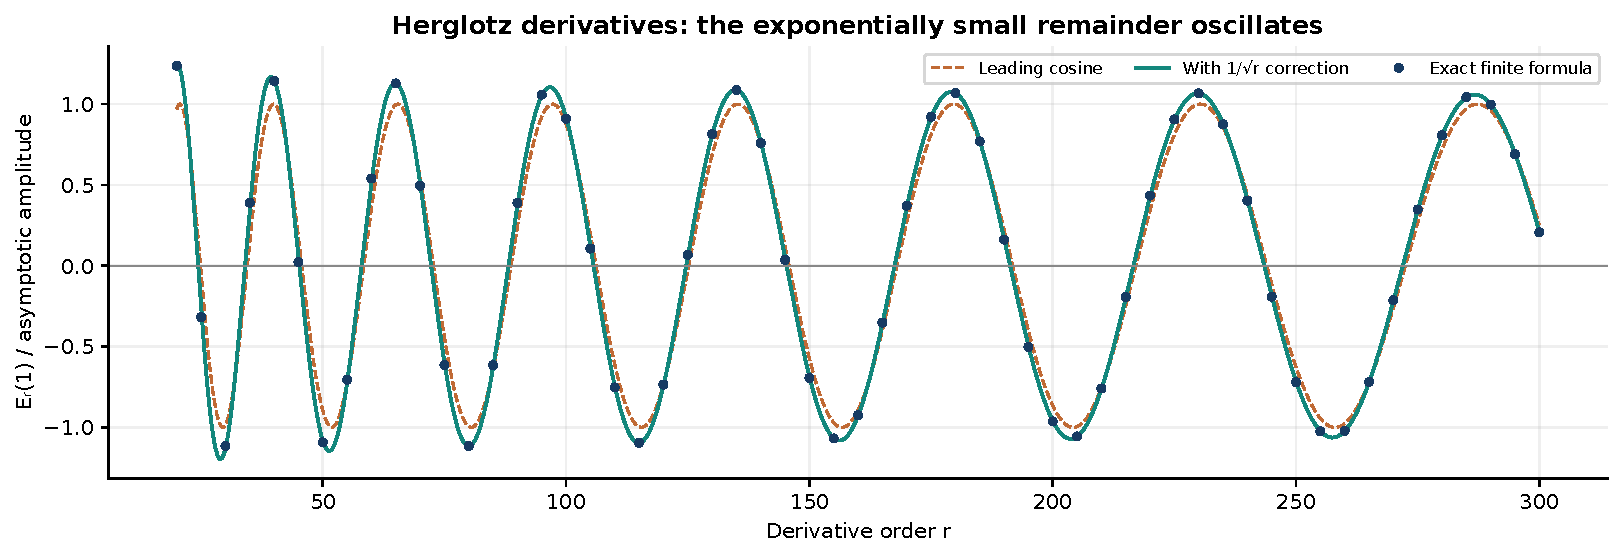
\includegraphics[width=\textwidth]{figures/herglotz_oscillation.pdf}
\caption{The Herglotz remainder divided by its asymptotic amplitude at $x=1$. The leading cosine and its first correction track the exact finite-formula values. The asymptotic is additive, so no division by a small cosine is used.}
\label{fig:herglotz}
\end{figure}

\section[Cyclotomic double relations: exact identities and formal obstructions]{Cyclotomic double relations:\\exact identities and formal obstructions}
\label{sec:gaussian}

Set
\[
 g_{a,b}=\Impart\Li_{a,b}(\ii,1),\quad
 A_{a,b}=\Impart\Li_{a,b}(\ii,\ii),\quad
 K_{a,b}=\Impart\Li_{a,b}(\ii,-1).
\]
The manuscript's mixed harmonic sums are
\[
 S_p=\sum_{n\geq0}\frac{(-1)^nH_n}{(2n+1)^p},\qquad p\geq1.
\]
For \(p>1\) this converges absolutely; at \(p=1\) it converges
conditionally. The all-odd-index evaluation of \(S_p\) has already
been proved in the repository's continuations. Our questions concern
even indices and what exact relations can establish about them.

\subsection{Two exact weight-five reductions}

\begin{proposition}[Two coordinates suffice for the weight-five \(g\)-family]
\label{prop:two-g}
The four values of weight five satisfy
\begin{align}
 g_{2,3}+3g_{3,2}+6g_{4,1}
   &=-\frac3{32}G\zeta(3)-\frac{\pi^5}{1536},
     \label{eq:g-five-first}\\
 g_{1,4}+g_{2,3}+g_{3,2}+2g_{4,1}
   &=-\frac12\beta(4)\log2-\frac{7\pi^5}{46080}.
     \label{eq:g-five-second}
\end{align}
Thus they lie in the span of any two suitably chosen coordinates,
for example \(g_{4,1},g_{2,3}\), together with the displayed products
of single values. This is a spanning statement, not an independence
statement.
\end{proposition}

\begin{proof}
Shuffle the two iterated-integral words for
\(\Li_2(\ii)\Li_3(\ii)\). Their imaginary part is
\(g_{2,3}+3g_{3,2}+6g_{4,1}\).
Since
\[
 \Li_2(\ii)=-\frac{\zeta(2)}8+\ii G,\qquad
 \Li_3(\ii)=-\frac{3\zeta(3)}{32}+\ii\frac{\pi^3}{32},
\]
its product gives \eqref{eq:g-five-first}.
Likewise, the shuffle of \(\Li_1(\ii)\Li_4(\ii)\) has imaginary part
\(g_{1,4}+g_{2,3}+g_{3,2}+2g_{4,1}\). Use
\[
 \Li_1(\ii)=-\tfrac12\log2+\ii\tfrac\pi4,\qquad
 \Li_4(\ii)=-\tfrac7{128}\zeta(4)+\ii\beta(4).
\]
The two rows have rank two already in their \(g\)-coefficients.
\end{proof}

The manuscript's displayed sporadic row
\[
 576g_{4,1}+288g_{3,2}+736g_{2,3}+960g_{1,4}
 =21G\zeta(3)-480\beta(4)\log2
\]
is \(-224\) times \eqref{eq:g-five-first} plus \(960\) times
\eqref{eq:g-five-second}. It therefore has a direct proof from
these two elementary shuffles. The manuscript's \emph{at most three}
statement can be strengthened to \emph{at most two}. Existing
continuations already address proofs of the sporadic relation; the
point here is the sharper two-row organization.

\subsection{An all-exponent mixed endpoint identity}

\begin{theorem}[Gaussian mixed endpoint]\label{thm:mixed-endpoint}
For every integer \(p\geq1\),
\begin{equation}\label{eq:mixed-endpoint}
 K_{p,1}+(-1)^{p-1}A_{1,p}
 =\beta(p+1)-2\log2\,\beta(p)
       +\sum_{j=2}^{p}(-1)^j\eta(j)\beta(p+1-j).
\end{equation}
Moreover,
\begin{equation}\label{eq:harmonic-split}
 S_p=g_{p,1}+K_{p,1}.
\end{equation}
\end{theorem}

\begin{proof}
All the boundary values used here converge. First-index-one values
with first argument \(\ii\) can be obtained by Dirichlet's test or
radial Abel limits. The shuffle and stuffle identities may therefore
be justified by convergent iterated integrals and Abel limiting.

Fix \(w=p+1\), and define homogeneous generating polynomials of
degree \(w-2\):
\[
 \mathscr A(X,Y)=\sum_{a+b=w}A_{a,b}X^{a-1}Y^{b-1},
 \quad
 \mathscr K(X,Y)=\sum_{a+b=w}K_{a,b}X^{a-1}Y^{b-1}.
\]
Let \(\mathscr V\) denote the same polynomial for
\(\Impart\Li_{a,b}(-1,\ii)\), and put
\[
 P(X,Y)=\sum_{a+b=w}
  \Impart[\Li_a(-1)\Li_b(\ii)]X^{a-1}Y^{b-1},
 \qquad
 H(X,Y)=\sum_{a+b=w}X^{a-1}Y^{b-1}.
\]
Stuffle and shuffle respectively give
\[
 \mathscr V(X,Y)+\mathscr K(Y,X)=P(X,Y)+\beta(w)H(X,Y),
\]
\[
 \mathscr A(X+Y,X)-\mathscr V(X+Y,Y)=P(X,Y).
\]
The collision term in the first equation is
\(-\Impart\Li_w(-\ii)=\beta(w)\).
Eliminating \(\mathscr V\) yields
\[
 \mathscr K(U,V)=P(V-U,U)+P(V,U)+\beta(w)H(V,U)
                  -\mathscr A(V,V-U).
\]
Set \(V=0\) and compare coefficients of \(U^{w-2}\).
The evaluation \(\Li_j(-1)=-\eta(j)\) gives
\eqref{eq:mixed-endpoint}, including the two occurrences of
\(-\log2\,\beta(p)\).

For \eqref{eq:harmonic-split}, taking imaginary parts of the outer
index in \(\Li_{p,1}(\ii,1)+\Li_{p,1}(\ii,-1)\) retains indices
\(2n+1\), with sign \((-1)^n\). Their inner sum is
\[
 \sum_{m=1}^{2n}\frac{1+(-1)^m}{m}=H_n.
\]
Absolute convergence proves the result directly for \(p>1\).
An Abel limit gives the endpoint \(p=1\).
\end{proof}

At \(p=4\) this specializes to
\begin{equation}\label{eq:K41}
 K_{4,1}=A_{1,4}+\frac{191\pi^5}{23040}
                  -\frac34G\zeta(3)-2\beta(4)\log2.
\end{equation}

\subsection{Inverse-argument mixed values and a source correction}

A useful regularization identity also removes a specific proposed
mixed survivor from the manuscript. Inverse-argument double reductions
are part of the existing repository programme; the following short
derivation makes the correction explicit.

\begin{proposition}[Inverse-argument endpoint]\label{prop:inverse-mixed}
For \(p\geq1\) and \(z=\ii\) or \(e^{2\pi\ii/3}\),
\begin{align}
 \Impart\Li_{p,1}(z,z^{-1})
 &=\sum_{a=1}^{p}\Impart\Li_{a,p+1-a}(z,1)
     +p\,\Impart\Li_{p+1}(z)\notag\\
 &\quad-\sum_{j=2}^{p}\zeta(j)\Impart\Li_{p+1-j}(z).
 \label{eq:inverse-mixed}
\end{align}
\end{proposition}

\begin{proof}
Give \(\Li_1(1)\) its usual real regularization parameter \(T\).
The shuffle expansion of \(T\Li_p(z)\) is
\[
 \Li_{p,1}(z,z^{-1})+\sum_{a=1}^{p}\Li_{a,p+1-a}(1,z),
\]
and its stuffle expansion is
\[
 \Li_{1,p}(1,z)+\Li_{p,1}(z,1)+\Li_{p+1}(z).
\]
The divergent leading term cancels on subtraction. For \(2\leq a\leq p\)
use the convergent stuffle
\[
 \Li_{a,p+1-a}(1,z)
 =\zeta(a)\Li_{p+1-a}(z)
       -\Li_{p+1-a,a}(z,1)-\Li_{p+1}(z).
\]
Taking imaginary parts gives \eqref{eq:inverse-mixed}.
For \(p=1\) there is only one divergent factor because \(z\ne1\);
the same cancellation proves the formula.
\end{proof}

Substitution of the already proved Gaussian weight-six \(g\)-values
gives the particularly short identity
\begin{equation}\label{eq:mixed-weight-six}
 \boxed{\displaystyle
 \Impart\Li_{5,1}(\ii,-\ii)
 =3\beta(6)-\frac{\pi^2}{6}\beta(4)
            -\frac{\pi^4}{90}G-\frac{5\pi^5}{3072}\log2.}
\end{equation}
Thus this imaginary weight-six value is in the depth-one product
basket. The candidate-survivor wording in Chapter~4 should be removed.

For \(\omega=e^{2\pi\ii/3}\), define
\(C_s=\Impart\Li_s(\omega)\); this is the sine-part convention for every
integer \(s\). Then
\begin{align}
 \Impart\Li_{5,1}(\omega,\omega^2)
 &=\sum_{a=1}^{5}\Impart\Li_{a,6-a}(\omega,1)
     +5C_6-\frac{\pi^2}{6}C_4-\frac{\pi^4}{90}C_2\notag\\
 &\quad-\frac{2\pi^3}{81}\zeta(3)-\frac{\pi}{6}\zeta(5).
 \label{eq:eisenstein-weight-six}
\end{align}
Here \(C_1=\pi/6\) and \(C_3=2\pi^3/81\).
It follows that the corresponding level-three imaginary value
contributes no new direction modulo the stated \(g\)-family and
single products. This conclusion says nothing about the manuscript's
real weight-five candidate.

\subsection{A precisely defined formal presentation}

Fix a level \(L=3\) or \(4\) and a weight \(w\geq2\). Let
\(\omega=e^{2\pi\ii/L}\).
Introduce rational formal symbols
\[
 D_a(r,s)\quad(1\leq a<w,\quad r,s\in\Z/L\Z)
\]
for imaginary parts of \(\Li_{a,w-a}(\omega^r,\omega^s)\).
Impose conjugation \(D_a(-r,-s)=-D_a(r,s)\).
Symbols fixed by this involution vanish. Put all single values and
imaginary parts of products of two single values in the background,
and also set \(D_a(1,0)=0\). The latter is precisely quotienting by
the chosen \(g\)-family.

The only further rows imposed are, for \(p+q=w\),
\begin{align}
 D_p(r,s)+D_q(s,r)&=0,\label{eq:formal-stuffle}\\
 \sum_{j=0}^{p-1}\binom{q+j-1}{j}D_{q+j}(s,r-s)
 +\sum_{j=0}^{q-1}\binom{p+j-1}{j}D_{p+j}(r,s-r)&=0.
 \label{eq:formal-shuffle}
\end{align}
They are the stuffle and shuffle rows of two single values, with their
one-leading-one regularizations. A regularized product involving the
real parameter \(T\) belongs to the background. At \(w=2\), the only
two-divergent-factor correction is real and disappears on taking
imaginary parts. Call the resulting quotient \(V_{L,w}\).

This is \emph{not} the full cyclotomic double-shuffle algebra. Products
involving a depth-two factor, relations lifted through higher depths,
additional functional equations, and motivic period assertions have
not been imposed. In particular, Zhao's standard relations
\cite{Zhao} are substantially broader than this presentation.
The theorem below computes \(V_{L,w}\), not a dimension of actual
numbers.

For a scalar assignment to the symbols, introduce
\[
 \mathscr F^{r,s}(X,Y)=
 \sum_{a=1}^{w-1}D_a(r,s)X^{a-1}Y^{w-a-1}.
\]
The conditions that the assignment annihilate all rows are exactly
\begin{align}
 \mathscr F^{r,s}(X,Y)+\mathscr F^{s,r}(Y,X)&=0,
 \label{eq:poly-stuffle}\\
 \mathscr F^{s,r-s}(X+Y,X)+
       \mathscr F^{r,s-r}(X+Y,Y)&=0.
 \label{eq:poly-shuffle}
\end{align}
These follow by comparing binomial coefficients after substitution.
They describe the dual of \(V_{L,w}\), so their solution dimension is
the required quotient dimension.

\subsection{All-weight dimension theorems}

\begin{theorem}[Level four]\label{thm:level-four}
The formal quotient satisfies
\[
 \dim_\Q V_{4,w}=
 \begin{cases}
 0,&w\ \text{even},\\
 (w-1)/2,&w\ \text{odd}.
 \end{cases}
 \qquad
 \sum_{w\geq2}\dim V_{4,w}\,t^w=\frac{t^3}{(1-t^2)^2}.
\]
At odd weight, its dual is parameterized by arbitrary antisymmetric
homogeneous polynomials of degree \(w-2\).
\end{theorem}

\begin{proof}
Up to conjugation, the six color pairs are
\((0,1),(1,0),(1,1),(1,2),(1,3),(2,1)\).
Write their polynomials as \(U,G,A,K,M,V\), respectively, and let
\(n=w-2\). The background condition gives \(G=0\);
stuffle gives
\[
 U=0,\quad A(Y,X)=-A(X,Y),\quad
 V(X,Y)=-K(Y,X),\quad M(Y,X)=M(X,Y).
\]
The shuffle with colors \((1,0)\) forces \(M=0\).
The shuffle with colors \((2,1)\) gives
\[
 A(X+Y,X)+K(Y,X+Y)=0,
\]
hence \(K(X,Y)=-A(Y,Y-X)\).
The shuffle with colors \((1,3)\) is
\(K(X,Y)=K(X,X-Y)\).
After substitution and antisymmetry this condition is
\(A=(-1)^{n+1}A\).

For even \(n\) all polynomials therefore vanish.
For odd \(n\), any antisymmetric \(A\), with \(K,V\) as above and
\(U=G=M=0\), satisfies the rows. To check exhaustiveness, the
unordered color classes up to conjugation are
\[
 (0,0),(0,1),(0,2),(1,1),(1,2),(1,3),(2,2).
\]
The real classes vanish, and the remaining classes are precisely the
conditions just used, together with their transposes. Thus there are
no unexamined rows.
A basis for \(A\) at odd \(w\) is
\[
 X^{a-1}Y^{w-a-1}-X^{w-a-1}Y^{a-1},
 \qquad 1\leq a\leq(w-1)/2.
\]
Counting these basis vectors and summing over odd weights proves
the formulas.
\end{proof}

\begin{theorem}[Level three]\label{thm:level-three}
The formal quotient satisfies
\[
 \dim_\Q V_{3,w}=
 \begin{cases}
 0,&w\ \text{even},\\
 \lfloor(w+1)/6\rfloor,&w\ \text{odd},
 \end{cases}
 \qquad
 \sum_{w\geq2}\dim V_{3,w}\,t^w
       =\frac{t^5}{(1-t^2)(1-t^6)}.
\]
Writing \(\Delta=XY(X-Y)\), \(Q=X^2-XY+Y^2\), the dual is parameterized
by the homogeneous polynomials
\[
 A(X,Y)=\Delta\,P(Q,\Delta^2)
\]
of degree \(w-2\).
\end{theorem}

\begin{proof}
Up to conjugation the four pairs are
\((0,1),(1,0),(1,1),(1,2)\).
As before the first two vanish and the shuffle with a zeta factor kills
the inverse-argument polynomial. The remaining polynomial \(A\)
satisfies exactly
\[
 A(Y,X)=-A(X,Y),\qquad A(X,X-Y)=A(X,Y).
\]
Antisymmetry implies divisibility by \(X-Y\); the second symmetry then
forces divisibility by \(Y\), and antisymmetry forces divisibility by
\(X\). Hence \(A=\Delta B\). The polynomial \(\Delta\) has the same
two transformation signs as \(A\), so \(B\) is invariant under swapping
\(X,Y\) and under \((X,Y)\mapsto(X,X-Y)\).

On the plane \(a+b+c=0\), with
\((a,b,c)=(X,-Y,Y-X)\), the second transformation swaps \(b,c\);
the first is global negation followed by the transposition of \(a,b\).
The generated group contains global negation, obtained by cubing
the product, and all permutations. The elementary symmetric-polynomial
theorem therefore identifies its invariant ring with
\[
 \Q[e_2,e_3^2]=\Q[Q,\Delta^2].
\]
Conversely every \(\Delta P(Q,\Delta^2)\) has the required symmetries,
and direct substitution verifies all the original color rows.
Counting monomials of degrees \(3+2a+6b=w-2\) gives the result.
Explicitly, at odd \(w\geq5\) a basis is
\[
 \Delta^{2b+1}Q^{(w-5)/2-3b},
 \qquad 0\leq b\leq\lfloor(w-5)/6\rfloor .
\]
\end{proof}

For comparison, the exact dimensions at the first few odd weights are
\[
\begin{array}{c|rrrrrrr}
 w&3&5&7&9&11&13&15\\ \hline
 \dim V_{3,w}&0&1&1&1&2&2&2\\
 \dim V_{4,w}&1&2&3&4&5&6&7
\end{array}
\]
and all even-weight dimensions are zero. The exact matrix script
checks both formulas through weight 16, including that the displayed
polynomial bases annihilate every raw row and have the stated rank.

\subsection{A separating functional for the \texorpdfstring{$S_4$}{S4} conjecture}

At every odd weight \(w\geq3\), choose
\(A(X,Y)=(Y-X)^{w-2}\) in the level-four theorem.
Then \(K(X,Y)=X^{w-2}\), \(V(X,Y)=-Y^{w-2}\).
This gives a rational linear functional \(\ell\) that annihilates every
defining row and every background value:
\begin{align}
 \ell(D_a(1,1))&=(-1)^{a+1}\binom{w-2}{a-1},\notag\\
 \ell(D_{w-1}(1,2))&=1,\qquad
 \ell(D_1(2,1))=-1. \label{eq:separating}
\end{align}
All other entries vanish, apart from conjugates with opposite signs.

At weight five its nonzero entries are particularly transparent:
\[
\begin{array}{c|rrrrrr}
 \text{symbol}&A_{1,4}&A_{2,3}&A_{3,2}&A_{4,1}
       &\Impart\Li_{1,4}(-1,\ii)&K_{4,1}\\ \hline
 \ell&1&-3&3&-1&-1&1
\end{array}
\]
The polynomial proof verifies all weights; the delivered certificate
also checks this six-entry vector against every exact weight-five row.

\begin{conjecture}[The manuscript's \(S_4\) identity]\label{conj:S4}
The following identity remains unproved in this continuation:
\begin{align}
 S_4&=\frac{4g_{4,1}-3g_{3,2}-9g_{2,3}}7
       +\frac{\pi^5}{224}-\frac{27}{224}G\zeta(3)
       -2\beta(4)\log2. \label{eq:S4-original}
\end{align}
\end{conjecture}

The exact identity \eqref{eq:K41} makes this equivalent to
\begin{equation}\label{eq:S4-A}
 161280A_{1,4}+69120(g_{4,1}+g_{3,2}+3g_{2,3})
       +617\pi^5-101520G\zeta(3)=0.
\end{equation}
The functional \(\ell\) sends its left side to \(161280\).
Consequently this relation does not follow from
\eqref{eq:formal-stuffle}--\eqref{eq:formal-shuffle} and the stated
background alone. This is an exact obstruction to a specific proof
strategy. Additional true analytic relations may still prove it.

Using \eqref{eq:g-five-first}, an equivalent version with only two
\(g\)-coordinates is
\begin{equation}\label{eq:S4-two}
 S_4=\frac{10g_{4,1}-8g_{2,3}}7
       +\frac{7\pi^5}{1536}-\frac3{28}G\zeta(3)
       -2\beta(4)\log2.
\end{equation}
All three displayed candidates are equivalent by proved identities;
none is silently promoted to a theorem.

\subsection{A new weight-seven candidate}

\begin{conjecture}[A reduction for \(S_6\)]\label{conj:S6}
With the same definitions,
\begin{align}
 S_6={}&\frac{722}{527}g_{6,1}
       +\frac{40}{527}g_{4,3}
       -\frac{128}{155}g_{2,5}
       +\frac{15191}{28569600}\pi^7\notag\\
      &-\frac3{124}G\zeta(5)
       -\frac{2373}{10540}\beta(4)\zeta(3)
       -2\beta(6)\log2. \label{eq:S6}
\end{align}
\end{conjecture}

The candidate was found in the ordered basket
\[
 (S_6,g_{6,1},g_{4,3},g_{2,5},\pi^7,
          G\zeta(5),\beta(4)\zeta(3),\beta(6)\log2).
\]
Its primitive integer relation vector is
\[
 \begin{split}
 (&485683200,-665395200,-36864000,401080320,\\
  &-258247,11750400,109347840,971366400).
 \end{split}
\]
A 100-digit search used coefficient bound \(10^{12}\) and tolerance
\(10^{-90}\). After the coefficients were frozen, reevaluation by
Mellin integrals at 220 working digits gave an integer-normalized
residual of approximately \(-2.315\times10^{-213}\).
An independent Euler transformation of the defining alternating
series, using 900 terms and 300 working digits, gave approximately
\(2.854\times10^{-263}\). The script records the full values and
the exact integer vector. These are numerical evidence, not a proof
or an interval certificate.

For the second method, the defining series are
\[
 g_{a,b}=\sum_{n\geq0}
       \frac{(-1)^nH_{2n}^{(b)}}{(2n+1)^a},
 \qquad H_m^{(b)}=\sum_{j=1}^{m}j^{-b},
\]
and the analogous series with \(H_n\) for \(S_6\).
Thus the second evaluation does not reuse the discovery integral.
Last transformed terms are recorded as diagnostics; their small
size alone is not asserted to bound the complete tail.

The weight-seven functional \eqref{eq:separating} sends the
integer-normalized candidate to \(485683200\). Its proof therefore
also requires information beyond the restricted single-product
presentation. A useful next step is to obtain a functional equation
that proves both \eqref{eq:S4-original} and \eqref{eq:S6}, with the
nonzero functional serving as a check that the missing relation has
actually been introduced.


\subsection{A rigorous rational certificate for the new conjecture}

The floating-point checks above can be strengthened to an exact
residual enclosure without resolving the equality itself.

\begin{theorem}[Euler remainder for harmonic numerators]\label{thm:euler-certificate}
Let \(a,b,q\) be positive integers,
\(c_n=H_{qn}^{(b)}/(2n+1)^a\), and
\(L=\sum_{n\geq0}(-1)^nc_n\).
Define \(\Delta c_n=c_{n+1}-c_n\) and
\[
 E_N=\sum_{k=0}^{N-1}\frac{(-\Delta)^k c_0}{2^{k+1}},
 \qquad N\geq1.
\]
Then
\begin{equation}\label{eq:euler-harmonic-bound}
 0\leq E_N-L\leq (N+1)2^{-N}c_1
     =(N+1)2^{-N}\frac{H_q^{(b)}}{3^a}.
\end{equation}
\end{theorem}

\begin{proof}
On the unit square use the positive measure
\[
 \dd\mu(t,u)=
 \frac{(-\log t)^{a-1}(-\log u)^{b-1}}
 {(a-1)!(b-1)!(1-u)}\dd t\,\dd u.
\]
Set \(v=t^2\), \(z=t^2u^q\). Integral representations for reciprocal
integer powers give
\[
 c_n=\int(v^n-z^n)\dd\mu,\qquad
 \int(v-z)\dd\mu=c_1<\infty.
\]
The measure itself need not have finite mass. All differences below
are integrable because they are bounded by a constant times \(v-z\).
For \(k\geq1\),
\[
 (-\Delta)^k c_0
 =\int[(1-v)^k-(1-z)^k]\dd\mu\leq0,\qquad
 |(-\Delta)^k c_0|\leq k c_1.
\]
Thus the Euler series converges absolutely.
It equals \(L\): introduce an Abel factor into the original series,
sum the geometric differences under an integrable bound, and let
the factor increase to 1. The ordinary series converges absolutely
for \(a>1\). When \(a=1\), its magnitudes eventually decrease to zero:
the harmonic increment divided by \(H_{qn}^{(b)}\) is
\(O(1/(n\log n))\) for \(b=1\) and \(O(n^{-b})\) for \(b>1\),
whereas the denominator ratio is \(1+2/(2n+1)\).
Abel's theorem identifies the limits.
Every omitted Euler term is nonpositive, and
\[
 \sum_{k=N}^{\infty}\frac{k}{2^{k+1}}=(N+1)2^{-N}.
\]
This proves both the sign and the bound.
\end{proof}

The finite sum has the exact rational form
\begin{equation}\label{eq:finite-euler-integer}
 E_N=2^{-N}\sum_{n=0}^{N-1}(-1)^nc_n
             \sum_{j=n+1}^{N}\binom Nj.
\end{equation}
Indeed,
\(\sum_{k=n}^{N-1}\binom{k}{n}2^{-k-1}
=2^{-N}\sum_{j=n+1}^{N}\binom Nj\).
When \(q=1\) or \(2\), a common denominator is
\(2^N\operatorname{lcm}(1,2,\ldots,2N)^{a+b}\).
Thus all four nonclassical constants in the \(S_6\) basket have
rapid exact rational enclosures.

For \(c_n=(dn+1)^{-s}\), \(d=1\) or \(2\), a positive
moment measure of total mass 1 instead gives
\(0\leq L-E_N\leq2^{-N}\).
This encloses \(\eta(s)\), \(\beta(s)\), and hence
\(\zeta(3),\zeta(5),\log2\) using rational factors.
For \(\pi\) use Machin's identity
\[
 \pi=16\arctan(1/5)-4\arctan(1/239)
\]
and the alternating-series bound for each arctangent.

The delivered standard-library script \texttt{certify\_s6.py} uses
\(N=900\), 240 arctangent terms at \(1/5\), and 80 at \(1/239\).
It performs every interval operation with integers and rational
fractions, and rounds final decimal endpoints outward.
The resulting integer-normalized residual \(R_6\) satisfies the
deliberately widened, easily readable rational enclosure
\begin{equation}\label{eq:S6-certificate}
 -5.016\times10^{-261}\leq R_6\leq3.845\times10^{-262}.
\end{equation}
The full 280-place endpoints are recorded in the JSON certificate.
The exact arithmetic gate checks, in particular,
\[
 \boxed{|R_6|<10^{-260}.}
\]
This is a rigorous error statement about the residual.
It is still not a proof that the residual equals zero.


\section{The cubic log-gamma moment: a classical evaluation and a source correction}
\label{sec:cubic}

Write
\[
 a=\frac12\log(2\pi),\qquad A=\gamma+\log(2\pi),\qquad
 M_j=\int_0^1\log^j\Gamma(x)\,dx.
\]
The manuscript's statement that identifying a named depth-two atom for $M_3$
is open requires correction.  Bailey, D.~Borwein, and J.~M.~Borwein evaluated
$M_3$ using derivatives of Tornheim--Witten zeta functions in Theorem~6,
equation~(61), of their 2015 paper~\cite{BBB}.  The author-hosted preprint is dated
27 June 2012.  Their formula does not establish a reduction to a prescribed
finite collection of ordinary zeta values and derivatives.  That more
restrictive question should be kept distinct from the already established
Tornheim evaluation.  The argument below independently derives an equivalent
formula and supplies a convenient convergence justification.

For complex parameters in an open neighbourhood of $(1,1,1)$, define
\[
 T(s,t,u)=\sum_{m,n\ge1}\frac1{m^s n^t(m+n)^u},
 \qquad T_j=\partial_jT,\quad T_{ij}=\partial_i\partial_jT.
\]
Every derivative below is evaluated at $(1,1,1)$ unless arguments are shown.
The notation $T_{12}$ and $T_{13}$ is preferable to an unqualified prime,
because different parameter derivatives give different constants.

\begin{theorem}[Classical cubic evaluation, with a direct proof]
Set
\[
 V=\frac{\pi^2}{48}+\frac{A^2}{12}
       -\frac{A\zeta'(2)}{\pi^2}+\frac{\zeta''(2)}{2\pi^2}.
\]
Then
\begin{equation}\label{cubic:main}
 \boxed{\displaystyle
 M_3=a^3+3aV+\frac{3\zeta(3)}{16}
 +\frac{3}{8\pi^2}
   \left(2A^2\zeta(3)-2A T_3+2T_{13}-T_{12}\right).}
\end{equation}
All derivatives on the right are represented by absolutely convergent
double series.  In particular, no analytic continuation or summation
prescription is needed to define these constants.
\end{theorem}

\begin{proof}
Let $f(x)=\log\Gamma(x)$, regarded as an integrable periodic function.
Since $f(x)=-\log x+O(x)$ as $x\downarrow0$ and $f$ is bounded near $1$,
we have $f\in L^p(0,1)$ for every finite $p\ge1$.
Kummer's Fourier expansion gives
\[
 f(x)=a+\sum_{n\ge1}
 \left(\frac{\cos(2\pi nx)}{2n}
       +\frac{A+\log n}{\pi n}\sin(2\pi nx)\right),
 \qquad 0<x<1.
\]
Equivalently, the positive Fourier coefficients are
\[
 h_n=\frac1n\left(\frac14-
                   \frac{i(A+\log n)}{2\pi}\right),
 \qquad h_{-n}=\overline{h_n}.
\]
For $0<r<1$, let $f_r$ be the Poisson mean of $f$, so that the coefficient
$h_n$ is replaced by $r^{|n|}h_n$.  The Fourier series is now absolutely
convergent, and Poisson approximate-identity convergence gives
$f_r\to f$ in $L^3$.  Consequently $\int f_r^j\to\int f^j$ for $j=1,2,3$:
for the cubic case this follows, for example, from
\[
 \|u^3-v^3\|_1\le\|u-v\|_3
       (\|u\|_3^2+\|u\|_3\|v\|_3+\|v\|_3^2).
\]

Write $g=f-a$. Orthogonality first gives
\begin{align*}
 \int_0^1g(x)^2\,dx
 &=2\sum_{n\ge1}|h_n|^2\\
 &=\frac{\zeta(2)}8+
   \frac{A^2\zeta(2)-2A\zeta'(2)+\zeta''(2)}{2\pi^2}=V.
\end{align*}
For the cube, a zero-sum triple of nonzero Fourier frequencies has two
positive frequencies $m,n$ and one negative frequency $-(m+n)$, or the
opposite signs.  Accounting for the three positions of the exceptional
sign and then conjugation gives
\begin{equation}\label{cubic:resonance}
 \int_0^1g_r(x)^3\,dx
 =6\mathop{\rm Re}\sum_{m,n\ge1}
     r^{2(m+n)}h_mh_n\overline{h_{m+n}}.
\end{equation}
The factor is correct also when $m=n$: the ordered double sum accounts
for the interchange of the two positive frequencies only when they differ.

These resonant sums converge absolutely at $r=1$. Indeed,
\[
 \sum_{m=1}^{k-1}\frac1{m(k-m)k}
       =\frac{2H_{k-1}}{k^2},
\]
and $|h_mh_nh_{m+n}|$ is bounded by a constant times
$(1+\log(m+n))^3/[mn(m+n)]$.  The grouped majorant is
$O((1+\log k)^4/k^2)$, which is summable.  Dominated convergence therefore
permits $r\uparrow1$ in \eqref{cubic:resonance}.

Put $p=1/4$ and $q_j=(A+\log j)/(2\pi)$.  Direct multiplication yields
\[
 \mathop{\rm Re}\bigl[(p-iq_m)(p-iq_n)(p+iq_{m+n})\bigr]
 =p^3+p(q_mq_{m+n}+q_nq_{m+n}-q_mq_n).
\]
The numerator in the second term is, apart from $4\pi^2$,
\[
 A^2+2A\log(m+n)+\log m\log(m+n)+\log n\log(m+n)-\log m\log n.
\]
By the definitions of the Tornheim derivatives, symmetry in $m,n$,
and $T(1,1,1)=2\zeta(3)$, we obtain
\[
 \int_0^1g(x)^3\,dx
 =\frac{3\zeta(3)}{16}
 +\frac{3}{8\pi^2}
       \bigl(2A^2\zeta(3)-2AT_3+2T_{13}-T_{12}\bigr).
\]
Finally, $\int g=0$ and $\int f^3=a^3+3a\int g^2+\int g^3$.
\end{proof}

\paragraph{Holomorphy and differentiation.}
For completeness, local holomorphy is also elementary.  If each real part
of $s,t,u$ is at least $1-\epsilon$, with $0<\epsilon<1/3$, grouping by
$k=m+n$ and splitting at $m=k/2$ gives a locally uniform majorant of order
$k^{-2+3\epsilon}$.  The sum converges uniformly on compact subsets of
such a neighbourhood.  Standard termwise differentiation therefore applies.
Alternatively, at $(1,1,1)$ any prescribed logarithmic numerator of degree
$d$ is dominated by $2H_{k-1}(\log k)^d/k^2$ after grouping.  These are
ordinary convergent derivatives; Abel means are used only to justify the
Fourier multiplication.

\paragraph{Relations to Euler double zeta derivatives.}
Define $Z(s)=\zeta(s,1)=\sum_{k\ge2}H_{k-1}k^{-s}$, so that the prime
in $Z'(2)$ differentiates its first argument.  Then
\begin{equation}\label{cubic:firstpartials}
 T(1,1,u)=2Z(u+1),\qquad
 T_3=2Z'(2),\qquad T_1=T_2=Z'(2)+\zeta'(3).
\end{equation}
The first identity follows from $1/[m(k-m)]=(1/m+1/(k-m))/k$.
For the last identity, use
$\sum_{n\ge1}1/[n(m+n)]=H_m/m$.
Equation~\eqref{cubic:main} thus exactly matches the published cubic formula.
It also makes clear why a search involving only ordinary Riemann-zeta
derivatives need not find a relation.  Failure of a finite PSLQ search
does not prove that such a reduction is impossible.

\subsection{A positive summand form and an explicit tail bound}

The combination in \eqref{cubic:main} can be computed without cancellation
between separate Tornheim constants.  For $k=m+n$, define
\[
 R_A(m,n)=A^2+2A\log k+\log m\log k+\log n\log k-\log m\log n.
\]
Since $A>0$, $\log k\ge\log m,\log n\ge0$, we have $R_A(m,n)>0$.
Writing $p=\log m,q=\log n,r=\log k$, one also has
$r(p+q)-pq\le r^2$: for fixed $r$, the expression is increasing separately
in $p,q\in[0,r]$.  Consequently
\[
 0<R_A(m,n)\le(A+\log k)^2.
\]
Therefore the diagonal partial sums
\[
 C_N=\frac3{32}\sum_{m+n\le N}\frac1{mn(m+n)}
    +\frac{3}{8\pi^2}
       \sum_{m+n\le N}\frac{R_A(m,n)}{mn(m+n)}
\]
increase to the centered cubic moment $M_3-a^3-3aV$.  Moreover,
\begin{align*}
 0<(M_3-a^3-3aV)-C_N
 &\le\sum_{k>N}\frac{2(1+\log k)}{k^2}
       \left(\frac3{32}+\frac{3(A+\log k)^2}{8\pi^2}\right).
\end{align*}
This gives a transparent computable enclosure, although its convergence
is only $O(\log^3N/N)$.  An integral bound may be used once the explicit
summand is decreasing; direct summation can handle the finite initial range.
This positivity observation is an immediate corollary of the Fourier
calculation, not a claim of a new classical-constant evaluation.

\subsection{Exponentially convergent numerical reproduction}

For $t>0$, put
\[
 C(t)=\operatorname{Li}_1(e^{-t})=-\log(1-e^{-t}),\qquad
 F(t)=\left.\partial_s\operatorname{Li}_s(e^{-t})\right|_{s=1}.
\]
The usual Mellin representation of the Tornheim sum gives
\begin{equation}\label{cubic:mellinpartials}
 T_{12}=\int_0^\infty F(t)^2\,dt,\quad
 T_{13}=\int_0^\infty F(t)C(t)(\log t+\gamma)\,dt,\quad
 T_3=\int_0^\infty C(t)^2(\log t+\gamma)\,dt.
\end{equation}
For $0<t<2\pi$, cancellation of the two poles in Jonqui\`ere's expansion
produces
\begin{align*}
 C(t)&=-\log t+\sum_{k\ge1}c_kt^k,
 &c_k&=\frac{(-1)^k\zeta(1-k)}{k!},\\
 F(t)&=-\alpha-\gamma\log t-\tfrac12\log^2t+\sum_{k\ge1}b_kt^k,
 &b_k&=\frac{(-1)^k\zeta'(1-k)}{k!},\\
 \alpha&=\gamma_1+\frac{\gamma^2}2+\frac{\pi^2}{12}.
\end{align*}
Here the Stieltjes convention is
$\zeta(1+z)=z^{-1}+\sum_{j\ge0}(-1)^j\gamma_jz^j/j!$.
For computational stability the coefficient formulas can be rewritten as
\begin{align*}
 c_1&=\tfrac12,&b_1&=\tfrac12\log(2\pi),\\
 c_{2j}&=\frac{(-1)^j\zeta(2j)}{j(2\pi)^{2j}},&
 b_{2j}&=c_{2j}\left(\log(2\pi)-\psi(2j)-\frac{\zeta'(2j)}{\zeta(2j)}\right),\\
 c_{2j+1}&=0\quad(j\ge1),&
 b_{2j+1}&=\frac{(-1)^{j+1}\pi\zeta(2j+1)}{(2j+1)(2\pi)^{2j+1}}
 \quad(j\ge1).
\end{align*}
The functional equation of the Riemann zeta function proves these identities.
Elementary bounds $\zeta(k)<2$, $|\zeta'(k)|<2$, $H_{k-1}\le k-1$,
$\gamma<1$, $\log(2\pi)<2$, and $2\pi>6$ give, for $k\ge2$,
\[
 |b_k|\le12\,6^{-k},\qquad |c_k|\le2\,6^{-k}.
\]
Thus after degree $K\ge1$ their remainders on $0<t\le1$ are at most
\[
 \epsilon_b=\frac{12}{5}6^{-K},\qquad
 \epsilon_c=\frac25 6^{-K}.
\]
All integrals of the resulting polynomials in $t$ and $\log t$ are evaluated
using $\int_0^1t^k\log^jt\,dt=(-1)^jj!/(k+1)^{j+1}$.

On $t\ge1$, insert
$C(t)=\sum_{n\ge1}e^{-nt}/n$ and
$F(t)=-\sum_{n\ge1}(\log n)e^{-nt}/n$.  The integral with the logarithmic
factor uses
\[
 \int_1^\infty e^{-kt}(\log t+\gamma)\,dt
 =\frac{E_1(k)+\gamma e^{-k}}k.
\]
Truncate this sum at $m+n\le N$.  A common upper bound for the three
omitted tails is
\[
 B_N=4\sum_{k>N}ke^{-k}
 =\frac{4e^{-(N+1)}((N+1)-Ne^{-1})}{(1-e^{-1})^2}.
\]
For the three integrals in the order $T_{12},T_{13},T_3$, safe total
series-truncation bounds are respectively
\[
 \epsilon_b(12+\epsilon_b)+B_N,\qquad
 5\epsilon_b+15\epsilon_c+2\epsilon_b\epsilon_c+B_N,\qquad
 10\epsilon_c+2\epsilon_c^2+B_N.
\]
For example the elementary estimates
$C(t)\le-\log t+1$ and
$|F(t)|\le4-\log t+\tfrac12\log^2t$ on $(0,1]$ imply all the constants
above.  The sharper bound $\int_0^1|F(t)|dt<6$ follows directly from its
coefficient expansion (one may use $0<\alpha<2$).
An elementary verification of the latter constant bound is available:
the defining limit for $\gamma_1$ and the total variation of
$x\mapsto\log x/x$ on $[1,\infty)$ give $|\gamma_1|\le2/e<3/4$;
combine this with $0<\gamma<3/5$ and $3<\pi<\sqrt{12}$.
This is an analytic truncation certificate; floating-point rounding must
be handled separately to turn an implementation into interval arithmetic.

The independent implementation \texttt{verify\_tornheim.py} evaluates the
three partials and compares \eqref{cubic:main} against direct log-gamma
quadrature.  Its output explicitly labels the rounding qualification.

\subsection{A sign check for an auxiliary identity}

If the June 2012 preprint is used, an auxiliary sign should be checked
before copying its Remark~3.  Put
\[
 S_\gamma=\sum_{m,n\ge1}
        \frac{(\gamma+\log m)(\gamma+\log n)}{mn(m+n)}.
\]
Directly expanding the numerator, with absolutely convergent sums, gives
\[
 T_{12}=S_\gamma+2\gamma\bigl(Z'(2)+\zeta'(3)\bigr)
                  -2\gamma^2\zeta(3).
\]
The coefficient of $S_\gamma$ is positive.  The displayed minus sign in
equations~(63) and~(65) of the author-hosted June 2012 preprint would make
their right side negative, although $T_{12}>0$.  This issue does not
affect the cubic formula proved above.  This note does not assert that
the same typographical error occurs in the final journal typesetting.


\section{Corrections, integration notes, and further research}
\label{sec:corrections}

\subsection{Proposed corrections to the pinned manuscript}

The following corrections are scoped to the pinned source, so that
a maintainer can distinguish a stale manuscript statement from a gap
in the repository as a whole. Some relevant identities are already
present in existing continuation material or its exact coefficient
code. The proposed patch updates a few local statements; this article
supplies the fuller proofs and context.

\paragraph{C1. The cubic moment has a named evaluation.}
Chapter~7, at \texttt{integral:neg:cubic}, calls the identification of a
named depth-two atom an open problem. Bailey--Borwein--Borwein
\cite[Theorem~6]{BBB} already provide a Tornheim--Witten derivative
evaluation. Replace that description by the formula in
Section~\ref{sec:cubic}, or a reference to it, and state the narrower
remaining problem: reduction of the prescribed derivative combination
to a specifically defined smaller basket. The cubic-moment discovery
paragraph in Chapter~10 should make the same distinction.
A failed numerical search in a smaller basket establishes no
nonmembership statement.

\paragraph{C2. Two weight-five coordinates suffice.}
The paragraph before \texttt{gauss:eq:S4-closed} in Chapter~4 infers
only an at-most-three spanning statement from its sporadic relation.
Proposition~\ref{prop:two-g} supplies two independent exact shuffle rows,
so at most two \(g\)-coordinates remain over the displayed single
products. The sporadic relation is a proved consequence. Its proof
status and its rank consequence should both be updated, while the
mixed \(S_4\) equation itself remains conjectural.

\paragraph{C3. The imaginary weight-six mixed survivors disappear.}
The statements around \texttt{mixed:sec:eisdim} and
\texttt{mixed:thm:parallel} propose imaginary weight-six mixed
directions at both levels. Equations~\eqref{eq:mixed-weight-six}
and~\eqref{eq:eisenstein-weight-six} give explicit reductions.
The all-weight inverse-argument coefficient function in the existing
report-10 code
\texttt{10-exact-structure-verify\_mixed\_and\_euler.py}
already contains the relevant reduction mechanism.
These manuscript survivor counts should therefore be revised.
The real weight-five question is unaffected by this argument and
should be treated separately.

\paragraph{C4. A coefficient label in the sixth-point proof.}
In Chapter~7's proof of \texttt{stieltjes:\allowbreak thm:\allowbreak G1half}, the text
describes
\(\log^2 6-\log^2 3-\log^2 2\) as a coefficient of \(\zeta''(0)\).
It is the coefficient of \(\zeta(0)\).
Indeed, for \(P(s)=6^s-3^s-2^s+1\),
\[
 P(0)=P'(0)=0,\qquad
 (P\zeta)''(0)=P''(0)\zeta(0)
       =(\log^2 6-\log^2 3-\log^2 2)\zeta(0).
\]
The displayed final identity in that proof is unchanged.

\paragraph{C5. Scope of dimension and independence language.}
All matrix-rank statements should specify the formal space, background
basket, convergence or regularization rules, and exact row family.
Theorems~\ref{thm:level-four} and~\ref{thm:level-three} provide such
a specification for one imaginary quotient. They do not validate
claims about the dimensions of all actual periods. Likewise,
non-reduction in a bounded-height search should be recorded as a
search result with the basket and bounds, not as a theorem of
arithmetic independence. The existing manuscript often gives this
warning; the surviving stronger wording should be made consistent.

\paragraph{C6. An auxiliary sign in a cited preprint.}
The June 2012 author-hosted version of \cite{BBB}, equations~(63)
and~(65), prints a minus sign before a manifestly positive quadratic
sum. Section~\ref{sec:cubic} gives a direct sign check and the corrected
plus sign. This observation is restricted to the inspected preprint.
It should not be generalized to an uninspected journal version.

\subsection{Integration and claim status}

A practical integration sequence is to update the short correction
paragraphs first, then add the quantitative moment and Herglotz
sections as separate research continuations, and finally replace
finite experimental dimension summaries by explicitly scoped theorems
where applicable. The selected \(S_6\) equation belongs in the
conjecture ledger with its frozen integer vector and exact residual
certificate.

The machine-readable \texttt{claim\_ledger.json} distinguishes
analytic theorems, exact formal-algebra theorems, classical
rederivations, source corrections, and unresolved conjectures.
The package excludes exploratory rejected candidates and does not
turn a small residual into an accepted identity. All paths needed
to rebuild the article are relative, and no repository-specific
absolute path is required by the LaTeX source.

\subsection{A proposed research programme}

The following questions have concrete starting points and distinct
success criteria. Their order reflects likely usefulness rather than
a claim that any is easy.

\begin{enumerate}[leftmargin=*,label=\textbf{R\arabic*.},itemsep=0.65em]

\item \textbf{Prove the two even-index harmonic reductions.}
Find a functional or iterated-integral relation proving
Conjecture~\ref{conj:S4} and then Conjecture~\ref{conj:S6}.
The separating functional shows that re-solving the same
single-product matrix cannot suffice. Candidate routes include
relations lifted through higher depth and the extra symmetries of
the level-four punctured sphere. A useful certificate would give
the new relation explicitly and show that its image under
\(\ell\) is nonzero before eliminating it with the other rows.
Zhao~\cite{Zhao} supplies relevant broader context, but the current
obstruction does not prove that any one of those routes is necessary.

\item \textbf{Determine an even-index family with a justified basket.}
For \(S_{2m}\), decide which \(g\)-coordinates and single products
are actually sufficient at each weight. The \(S_4\) and \(S_6\)
equations suggest structured reductions, but two examples do not
determine a general coefficient law. Choose the basket from exact
relations, freeze it, record a height bound before each search, and
validate any candidate with the rational Euler method.
The desired outcome is a uniform formula or a precise counterexample
to a proposed family, rather than an unqualified claim that odd
weights require new constants.

\item \textbf{Extend the formal quotient to other levels.}
Compute the analogue of \(V_{L,w}\) first for \(L=5\) and \(6\),
with exactly the same row conventions. Determine whether its
polynomial description comes from a finite group, a module over an
invariant ring, or a more complicated relation. An all-weight Hilbert
series should be accompanied by explicit spanning and separating
families, not inferred from a short table.

\item \textbf{Compare restricted and larger relation presentations.}
Add depth-two distribution, weight-one relations, and lifted
higher-depth rows in a documented order. At each step compute the
kernel induced on the polynomial parameters of
Theorems~\ref{thm:level-four} and~\ref{thm:level-three}.
This would show exactly which new rows remove which obstructions.
A later comparison with motivic bounds must keep formal dimension,
period dimension, and conditional period conjectures distinct.

\item \textbf{Uniform moment truncation beyond the least-term window.}
Theorem~\ref{thm:optimal-moment} treats bounded
\(\eta=N\Lambda-n\). Develop a uniform expansion when \(N/n\)
varies over a positive interval, and then when it tends to zero or
infinity. The inverse remainder kernel and gamma concentration
suggest the relevant starting formula. The challenge is to retain
uniform error estimates through the changing concentration region.
A second target is a fully explicit finite-\(n,N\) remainder bound.

\item \textbf{Global analytic structure of the inverse gamma branch.}
Locate the next singularities reached by analytic continuation of
the particular branch \(g\), including which critical values
actually lie on that branch. Determine their contributions after
the leading square-root expansion is removed. The local slit-disk
argument used here deliberately avoids an unsupported assertion
about a global inverse. Understanding the further singularities
could explain exponentially smaller corrections to the late
coefficients and constrain possible global sign bounds.

\item \textbf{Higher Herglotz corrections and transition in the argument.}
Compute several more half-integer terms in the oscillatory expansion
and give explicit error constants. More substantially, analyze
simultaneous limits such as \(x/r\to\xi>0\) or \(x\to0\) with \(r\).
The fixed-\(x\), compact-uniform theorem does not automatically cover
these regimes: the optimal Mellin contour and the contributing
arithmetic sectors change. A useful result would identify the
transition from one dominant sector to a collective contribution.

\item \textbf{Quantitative Herglotz sign locations.}
Theorem~\ref{thm:herglotz-oscillation} gives infinitely many signs,
but does not identify every sign for every large integer \(r\).
Use higher corrections and explicit bounds to locate the changes
near the zeros of the leading cosine. Because the phase increment
tends to zero, an additive error estimate is essential near these
zeros. The target is an eventually certified sign algorithm and an
asymptotic count of transitions.

\item \textbf{Arithmetic twists of the high-derivative theorem.}
Replace the divisor coefficients by character-twisted coefficients
or consider higher Herglotz functions. The functional-equation
framework of \cite{RZ,DSS} is a natural starting point.
Determine how parity, conductor, and vanishing of the first
arithmetic coefficient alter the exponential rate and oscillatory
phase. The sum of all sectors must again be bounded uniformly;
a single special-function asymptotic is not enough.

\item \textbf{Minimal derivative coordinates for the cubic moment.}
The cubic formula singles out \(2T_{13}-T_{12}\), together with
\(T_3=2Z'(2)\). Determine the exact relations among Tornheim
derivatives at \((1,1,1)\) obtained from symmetry, integration by
parts, and differentiated functional equations. State a candidate
basis before asking whether this combination reduces to ordinary
zeta derivatives. Failure of such a reduction search should not be
confused with the already solved problem of finding a named
depth-two representation.

\item \textbf{Certified evaluation of the asymptotic quantities.}
Combine the explicit tail estimates with interval implementations
of gamma, polygamma, Hurwitz zeta, and the remaining finite
integrals. For moments, the cutoff identity
\eqref{eq:cutoff} provides a convergent route; for Herglotz remainders,
\eqref{eq:herglotz-simple-tail} provides a simple arithmetic cutoff.
The rational \(S_6\) certificate is a model of the distinction between
a proved truncation bound and an actual certified implementation.

\item \textbf{Repository-level mathematical provenance.}
Attach to every accepted identity its exact normalization,
definition of the basis, proof source, executable check, and status.
For dimension claims also store the row generator and a basis or
separating witness. For numerical conjectures store the frozen
coefficients separately from discovery logs, with an independent
holdout computation. This would prevent a correction already
proved in a continuation from remaining an open claim in the
consolidated manuscript.

\end{enumerate}

These questions connect the analytic and algebraic sides of the
programme: good coordinates make strong conjectures visible, while
controlled remainders and explicit relation spaces show exactly
what has, and has not, been proved.


\section{Reproducibility, numerical evidence, and limitations}
\label{sec:verification}

The package includes the complete LaTeX source, generated figures, exact
relation-space code, numerical diagnostics, rational certificates, a
claim ledger, and a proposed source patch. Computations are separated
into exact arithmetic and ordinary high-precision arithmetic. The
analytic proofs are in the article; the numerical checks provide
independent diagnostics for constants, signs, branches, and truncation
scales.

\subsection{Moment coefficients and least-term errors}

The recurrence in Section~\ref{sec:moments} generates \(b_k\)
without numerically inverting gamma. The script
\texttt{verify\_moments.py} also checks the first eight coefficient
polynomials against a separate formal exponential-series expansion.
For direct moments it substitutes \(x=e^{-t}\) and integrates
\[
 m_n=\int_0^\infty
  \exp\bigl(n\log(\log\Gamma(e^{-t}))-t-\log\Gamma(n+1)\bigr)\dd t.
\]
The upper limit is infinity. A fixed short cutoff may approximate
\(m_n\) accurately while corrupting the far smaller least-term error,
so it is unsuitable for this check unless its tail is explicitly
controlled.

The computations use 180 decimal working digits. Orders 20 and 80
are repeated at 215 digits; the respective differences between
normalized remainder ratios are below \(3\times10^{-162}\) and
\(6\times10^{-67}\). The latter loses many digits through the
deliberate subtraction of a remainder of order \(10^{-113}\);
the extra precision is therefore material.

\begin{center}
\small
\begin{tabular}{rrrrr}
\toprule
\(n\)&\(N\)&\(\eta=N\Lambda-n\)&
error / first omitted term&
\(N^3\)(error after two corrections)\\
\midrule
10&9 &1.388939&0.503338844959&0.059202\\
20&17&1.512440&0.499910660977&0.056121\\
30&25&1.635941&0.498697774004&0.055539\\
40&33&1.759442&0.498075743812&0.052612\\
60&49&2.006443&0.497442625716&0.042058\\
80&64&0.988008&0.501995818744&0.046583\\
\bottomrule
\end{tabular}
\end{center}
The final column refers to the normalized ratio in
\eqref{eq:moment-second}, not to \(M_n\) itself.
The bounded values corroborate the predicted \(O(N^{-3})\) term;
they are not used to prove it.

\subsection{Herglotz derivatives}

The finite rational formula is compared against a separate positive
real integral at eight rational arguments and five derivative orders,
giving 40 comparisons. The maximum observed residual at 70 working
digits is about \(1.27\times10^{-70}\).
The coefficient construction uses exact SymPy Bernoulli polynomials;
the numerical integral uses independently generated Eulerian
coefficients for \(\Li_{1-r}\).

Seven higher-order checks, at \(r=10,20,30,50,80,100,150\), increase
working precision with the size of the Bernoulli sum and repeat at
40 additional digits. This avoids mistaking cancellation error for
the exponentially small \(E_r\). Selected values at \(x=1\) are
\[
\begin{array}{r|r}
 r&E_r(1)\\ \hline
 20& 9.5700353115338104\times10^{-8}\\
 30&-1.8039764729798573\times10^{-9}\\
 50&-4.2383422584491617\times10^{-12}\\
 100&6.4956183476241665\times10^{-17}\\
 150&-1.2668021540982769\times10^{-20}
\end{array}
\]
Three finite divisor-\(U\) sums are compared with the exact rational
derivative formula and both available analytic tail bounds.
Twelve checks of the single-sector saddle expansion cover
\(x=1/2,1,2\) and four derivative orders. The figure uses 57 further
exact-formula evaluations through \(r=300\), with precision chosen
to cover cancellation. These checks confirm the implementation and
the phase normalization; the sign theorem is analytic.

\subsection{Cyclotomic relation spaces and the conjecture certificate}

The exact row generator checks both levels through weight 16:
30 rational rank calculations, together with verification that
the proposed polynomial bases annihilate every row and have full
predicted rank. The weight-five separating functional is checked
entry by entry. The all-weight proofs in the article establish the
dimensions beyond that finite range.

Separate 90-digit integral diagnostics verify the two weight-five
shuffle rows, both versions of \(S_4\), its equivalent \(A_{1,4}\)
form, and the inverse-argument weight-six identities. Residuals for
the two \(S_4\) forms are about \(1.53\times10^{-92}\).
This is new corroboration of an existing conjecture, not its proof.

The \(S_6\) evidence has three independent layers: a 220-digit
Mellin-integral computation, a 300-digit Euler-series computation,
and an exact rational enclosure. The last uses only Python's
standard library and the proved tails in
Theorem~\ref{thm:euler-certificate}. It is therefore a certificate of
the bound \eqref{eq:S6-certificate}, including rounding, rather than
a heuristic precision report. The residual interval contains zero;
it cannot distinguish an exact identity from a sufficiently small
nonzero value.

\subsection{Reproduction of the classical cubic evaluation}

Using small-\(t\) degree 120, large-\(t\) diagonal cutoff 240, and
80 working digits, the Tornheim implementation gives
\begin{align*}
 T_3&=-4.85147944680912469492172639886220773949\ldots,\\
 T_{12}&=4.30244762034222643331985179818698942752\ldots,\\
 T_{13}&=8.71447281121431423816300785446242065162\ldots,\\
 M_3&=5.74038880722947428001957168810246146296\ldots.
\end{align*}
The direct moment integral and the Tornheim expression differ by
about \(1.69\times10^{-80}\).
The three analytic series-truncation bounds are respectively below
\(1.3\times10^{-92}\), \(7.6\times10^{-93}\), and
\(1.7\times10^{-93}\).
These bounds control series truncation, while the implementation's
floating-point rounding and quadrature remain separately qualified.
The mismatch between the sizes of the truncation bounds and the
observed residual is expected at 80-digit working precision.

\subsection{Running the package}

The root \texttt{README.md} and \texttt{Makefile} give the complete
commands. A typical sequence is
\begin{verbatim}
python3 -m pip install -r requirements.txt
make exact
make numeric
make figures
make pdf
\end{verbatim}
The exact \(S_6\) certificate alone requires no third-party package:
\begin{verbatim}
python3 scripts/certify_s6.py \
  --output data/s6_rational_certificate.json
\end{verbatim}
The PDF build uses ordinary \texttt{pdflatex}/\texttt{latexmk} and
standard TeX packages; its input figures are included.
All output data needed to inspect the delivered computations are
already present, so rerunning every numerical calculation is optional.

A source manifest pins the research baseline, and a SHA-256 manifest
covers the delivered artifacts. The correction patch is a proposal
for the pinned source; it should be reviewed against any newer
upstream revision before application. No external service is needed
to run the certificate, relation-space checks, or article build.


\begin{thebibliography}{99}

\bibitem{ProveIt}
V.~Reshetnikov and contributors,
\emph{ProveIt: Polylogarithms manuscript and research continuations}.
Source baseline: commit
\texttt{78f9e5df05eb0abb16c89fb00b9e89403598bd17}, 9 October 2026.
\url{https://github.com/VladimirReshetnikov/ProveIt/tree/78f9e5df05eb0abb16c89fb00b9e89403598bd17/Analysis/Polylogarithms/docs}.
Exact examined paths and content hashes are recorded in
\texttt{source\_manifest.json}.

\bibitem{ACEMKM}
T.~Amdeberhan, M.~W.~Coffey, O.~Espinosa, C.~Koutschan,
D.~V.~Manna, and V.~H.~Moll,
\emph{Integrals of powers of loggamma},
Proc. Amer. Math. Soc. \textbf{139} (2011), no.~2, 535--545.
\href{https://doi.org/10.1090/S0002-9939-2010-10589-0}
{doi:10.1090/S0002-9939-2010-10589-0}.
Author preprint:
\url{https://www.math.tulane.edu/~vhm/papers_html/lg-subm.pdf}.
Section~8 gives the classical moment expansion.

\bibitem{FS}
P.~Flajolet and R.~Sedgewick,
\emph{Analytic Combinatorics}, Cambridge University Press, 2009.
The smooth implicit-function schema and singularity transfer are the
classical background for the late-coefficient analysis.

\bibitem{BBB}
D.~H.~Bailey, D.~Borwein, and J.~M.~Borwein,
\emph{On Eulerian log-gamma integrals and Tornheim--Witten zeta functions},
Ramanujan J. \textbf{36} (2015), 43--68.
\href{https://doi.org/10.1007/s11139-012-9427-1}
{doi:10.1007/s11139-012-9427-1}.
Author-hosted preprint dated 27 June 2012:
\url{https://carmamaths.org/resources/jon/log-gamma.pdf}.
Theorem~6, equation~(61), is the cubic evaluation discussed here.
The auxiliary sign observation is scoped to this preprint's
equations~(63) and~(65).

\bibitem{RZ}
D.~Radchenko and D.~Zagier,
\emph{Arithmetic properties of the Herglotz function},
J. Reine Angew. Math. \textbf{797} (2023), 229--253.
\href{https://doi.org/10.1515/crelle-2023-0009}
{doi:10.1515/crelle-2023-0009}.
Author preprint:
\url{https://people.mpim-bonn.mpg.de/zagier/files/preprints/HerglotzFunction.pdf};
arXiv:2012.15805.
See equation~(6), the paragraph after Proposition~4, and Section~7.3.

\bibitem{DSS}
A.~Dixit, S.~Sathyanarayana, and N.~Guru Sharan,
\emph{Mordell--Tornheim zeta functions and functional equations for
Herglotz--Zagier type functions},
Adv. Math. \textbf{473} (2025), article 110303.
\href{https://doi.org/10.1016/j.aim.2025.110303}
{doi:10.1016/j.aim.2025.110303}.
Author preprint:
\url{https://adixit.people.iitgn.ac.in/wp/wp-content/uploads/2024/05/dss2.pdf};
arXiv:2405.07934.
The literature comparison in this continuation uses the accessible
author-hosted preprint.

\bibitem{Temme}
N.~M.~Temme,
\emph{Uniform asymptotic expansions of a class of integrals in terms of
modified Bessel functions, with application to confluent hypergeometric
functions},
SIAM J. Math. Anal. \textbf{21} (1990), no.~1, 241--261.
\href{https://doi.org/10.1137/0521013}{doi:10.1137/0521013}.

\bibitem{DLMF}
National Institute of Standards and Technology,
\emph{NIST Digital Library of Mathematical Functions},
Section~13.4, equation~13.4.4, and Section~13.8(iii),
equations~13.8.11--16.
\url{https://dlmf.nist.gov/13.4.E4};
\url{https://dlmf.nist.gov/13.8.iii}.
Consulted 9--10 October 2026.

\bibitem{Zhao}
J.~Zhao,
\emph{Multiple polylogarithm values at roots of unity},
C. R. Acad. Sci. Paris, Ser. I \textbf{346} (2008), 1029--1032.
\href{https://doi.org/10.1016/j.crma.2008.09.011}
{doi:10.1016/j.crma.2008.09.011}.
\url{https://www.numdam.org/item/10.1016/j.crma.2008.09.011.pdf}.
Its standard-relation framework includes more relations and depths
than the restricted presentation computed in this article.

\end{thebibliography}


\end{document}

